% Options for packages loaded elsewhere
\PassOptionsToPackage{unicode}{hyperref}
\PassOptionsToPackage{hyphens}{url}
%
\documentclass[
]{article}
\usepackage{lmodern}
\usepackage{amssymb,amsmath}
\usepackage{ifxetex,ifluatex}
\ifnum 0\ifxetex 1\fi\ifluatex 1\fi=0 % if pdftex
  \usepackage[T1]{fontenc}
  \usepackage[utf8]{inputenc}
  \usepackage{textcomp} % provide euro and other symbols
\else % if luatex or xetex
  \usepackage{unicode-math}
  \defaultfontfeatures{Scale=MatchLowercase}
  \defaultfontfeatures[\rmfamily]{Ligatures=TeX,Scale=1}
\fi
% Use upquote if available, for straight quotes in verbatim environments
\IfFileExists{upquote.sty}{\usepackage{upquote}}{}
\IfFileExists{microtype.sty}{% use microtype if available
  \usepackage[]{microtype}
  \UseMicrotypeSet[protrusion]{basicmath} % disable protrusion for tt fonts
}{}
\usepackage{xcolor}
\IfFileExists{xurl.sty}{\usepackage{xurl}}{} % add URL line breaks if available
\IfFileExists{bookmark.sty}{\usepackage{bookmark}}{\usepackage{hyperref}}
\hypersetup{
  pdftitle={Validation results},
  pdfauthor={Meg Cychosz},
  hidelinks,
  pdfcreator={LaTeX via pandoc}}
\urlstyle{same} % disable monospaced font for URLs
\usepackage[margin=1in]{geometry}
\usepackage{color}
\usepackage{fancyvrb}
\newcommand{\VerbBar}{|}
\newcommand{\VERB}{\Verb[commandchars=\\\{\}]}
\DefineVerbatimEnvironment{Highlighting}{Verbatim}{commandchars=\\\{\}}
% Add ',fontsize=\small' for more characters per line
\usepackage{framed}
\definecolor{shadecolor}{RGB}{248,248,248}
\newenvironment{Shaded}{\begin{snugshade}}{\end{snugshade}}
\newcommand{\AlertTok}[1]{\textcolor[rgb]{0.94,0.16,0.16}{#1}}
\newcommand{\AnnotationTok}[1]{\textcolor[rgb]{0.56,0.35,0.01}{\textbf{\textit{#1}}}}
\newcommand{\AttributeTok}[1]{\textcolor[rgb]{0.77,0.63,0.00}{#1}}
\newcommand{\BaseNTok}[1]{\textcolor[rgb]{0.00,0.00,0.81}{#1}}
\newcommand{\BuiltInTok}[1]{#1}
\newcommand{\CharTok}[1]{\textcolor[rgb]{0.31,0.60,0.02}{#1}}
\newcommand{\CommentTok}[1]{\textcolor[rgb]{0.56,0.35,0.01}{\textit{#1}}}
\newcommand{\CommentVarTok}[1]{\textcolor[rgb]{0.56,0.35,0.01}{\textbf{\textit{#1}}}}
\newcommand{\ConstantTok}[1]{\textcolor[rgb]{0.00,0.00,0.00}{#1}}
\newcommand{\ControlFlowTok}[1]{\textcolor[rgb]{0.13,0.29,0.53}{\textbf{#1}}}
\newcommand{\DataTypeTok}[1]{\textcolor[rgb]{0.13,0.29,0.53}{#1}}
\newcommand{\DecValTok}[1]{\textcolor[rgb]{0.00,0.00,0.81}{#1}}
\newcommand{\DocumentationTok}[1]{\textcolor[rgb]{0.56,0.35,0.01}{\textbf{\textit{#1}}}}
\newcommand{\ErrorTok}[1]{\textcolor[rgb]{0.64,0.00,0.00}{\textbf{#1}}}
\newcommand{\ExtensionTok}[1]{#1}
\newcommand{\FloatTok}[1]{\textcolor[rgb]{0.00,0.00,0.81}{#1}}
\newcommand{\FunctionTok}[1]{\textcolor[rgb]{0.00,0.00,0.00}{#1}}
\newcommand{\ImportTok}[1]{#1}
\newcommand{\InformationTok}[1]{\textcolor[rgb]{0.56,0.35,0.01}{\textbf{\textit{#1}}}}
\newcommand{\KeywordTok}[1]{\textcolor[rgb]{0.13,0.29,0.53}{\textbf{#1}}}
\newcommand{\NormalTok}[1]{#1}
\newcommand{\OperatorTok}[1]{\textcolor[rgb]{0.81,0.36,0.00}{\textbf{#1}}}
\newcommand{\OtherTok}[1]{\textcolor[rgb]{0.56,0.35,0.01}{#1}}
\newcommand{\PreprocessorTok}[1]{\textcolor[rgb]{0.56,0.35,0.01}{\textit{#1}}}
\newcommand{\RegionMarkerTok}[1]{#1}
\newcommand{\SpecialCharTok}[1]{\textcolor[rgb]{0.00,0.00,0.00}{#1}}
\newcommand{\SpecialStringTok}[1]{\textcolor[rgb]{0.31,0.60,0.02}{#1}}
\newcommand{\StringTok}[1]{\textcolor[rgb]{0.31,0.60,0.02}{#1}}
\newcommand{\VariableTok}[1]{\textcolor[rgb]{0.00,0.00,0.00}{#1}}
\newcommand{\VerbatimStringTok}[1]{\textcolor[rgb]{0.31,0.60,0.02}{#1}}
\newcommand{\WarningTok}[1]{\textcolor[rgb]{0.56,0.35,0.01}{\textbf{\textit{#1}}}}
\usepackage{longtable,booktabs}
% Correct order of tables after \paragraph or \subparagraph
\usepackage{etoolbox}
\makeatletter
\patchcmd\longtable{\par}{\if@noskipsec\mbox{}\fi\par}{}{}
\makeatother
% Allow footnotes in longtable head/foot
\IfFileExists{footnotehyper.sty}{\usepackage{footnotehyper}}{\usepackage{footnote}}
\makesavenoteenv{longtable}
\usepackage{graphicx,grffile}
\makeatletter
\def\maxwidth{\ifdim\Gin@nat@width>\linewidth\linewidth\else\Gin@nat@width\fi}
\def\maxheight{\ifdim\Gin@nat@height>\textheight\textheight\else\Gin@nat@height\fi}
\makeatother
% Scale images if necessary, so that they will not overflow the page
% margins by default, and it is still possible to overwrite the defaults
% using explicit options in \includegraphics[width, height, ...]{}
\setkeys{Gin}{width=\maxwidth,height=\maxheight,keepaspectratio}
% Set default figure placement to htbp
\makeatletter
\def\fps@figure{htbp}
\makeatother
\setlength{\emergencystretch}{3em} % prevent overfull lines
\providecommand{\tightlist}{%
  \setlength{\itemsep}{0pt}\setlength{\parskip}{0pt}}
\setcounter{secnumdepth}{5}
\usepackage{booktabs}
\usepackage{longtable}
\usepackage{array}
\usepackage{multirow}
\usepackage{wrapfig}
\usepackage{float}
\usepackage{colortbl}
\usepackage{pdflscape}
\usepackage{tabu}
\usepackage{threeparttable}
\usepackage{threeparttablex}
\usepackage[normalem]{ulem}
\usepackage{makecell}

\title{Validation results}
\author{Meg Cychosz}
\date{01 December 2020}

\begin{document}
\maketitle

\begin{Shaded}
\begin{Highlighting}[]
\CommentTok{# get total # of clips from each recording}
\NormalTok{complete2 <-}\StringTok{ }\NormalTok{complete }\OperatorTok\StringTok{ }
\StringTok{  }\KeywordTok{group_by}\NormalTok{(id) }\OperatorTok
\StringTok{  }\KeywordTok{distinct}\NormalTok{(file_name, }\DataTypeTok{.keep_all =}\NormalTok{ T) }\OperatorTok
\StringTok{  }\KeywordTok{mutate}\NormalTok{(}\DataTypeTok{num_clips =} \KeywordTok{NROW}\NormalTok{(Media)}\OperatorTok{*}\DecValTok{2}\NormalTok{) }

\NormalTok{clips <-}\StringTok{ }\NormalTok{complete2 }\OperatorTok
\StringTok{  }\KeywordTok{select}\NormalTok{(id, num_clips) }\OperatorTok\StringTok{ }
\StringTok{  }\KeywordTok{distinct}\NormalTok{(id, }\DataTypeTok{.keep_all =}\NormalTok{ T)}

\NormalTok{data <-}\StringTok{ }\KeywordTok{merge}\NormalTok{(clips, random, }\DataTypeTok{by=}\StringTok{'id'}\NormalTok{)}
\NormalTok{data2 <-}\StringTok{ }\KeywordTok{rbind}\NormalTok{(data, complete2)}
\end{Highlighting}
\end{Shaded}

\begin{Shaded}
\begin{Highlighting}[]
\NormalTok{data3 <-}\StringTok{ }\NormalTok{data2 }\OperatorTok
\StringTok{  }\KeywordTok{group_by}\NormalTok{(method, id) }\OperatorTok
\StringTok{  }\KeywordTok{mutate}\NormalTok{(}\DataTypeTok{num_clips_drawn =}\NormalTok{ (}\KeywordTok{NROW}\NormalTok{(file_name))) }\OperatorTok
\StringTok{  }\KeywordTok{mutate}\NormalTok{(}\DataTypeTok{percen_ofallclips_drawn=}\NormalTok{(}\KeywordTok{NROW}\NormalTok{(file_name)}\OperatorTok{/}\NormalTok{num_clips)}\OperatorTok{*}\DecValTok{100}\NormalTok{) }\CommentTok{# sanity check - complete method should be 50%}
\end{Highlighting}
\end{Shaded}

\begin{Shaded}
\begin{Highlighting}[]
\NormalTok{data_annon <-}\StringTok{ }\NormalTok{data3 }\OperatorTok
\StringTok{ }\KeywordTok{gather}\NormalTok{(}\StringTok{"addressee"}\NormalTok{, }\StringTok{"language"}\NormalTok{, Adult2OtherChild, Adult2Others, Adult2TargetChild, Adult2unsure, Otherchild2OtherChild, Otherchild2TargetChild, Otherchild2adults, Otherchild2unsure) }\OperatorTok
\StringTok{  }\KeywordTok{filter}\NormalTok{(language}\OperatorTok{==}\StringTok{'Mixed'} \OperatorTok{|}\StringTok{ }\NormalTok{language}\OperatorTok{==}\StringTok{'Spanish'} \OperatorTok{|}\StringTok{ }\NormalTok{language}\OperatorTok{==}\StringTok{'English/Quechua'} \OperatorTok{|}\StringTok{ }\NormalTok{language }\OperatorTok{==}\StringTok{'Unsure'}\NormalTok{) }\OperatorTok\StringTok{ }\CommentTok{# only clips w speech}
\StringTok{  }\KeywordTok{group_by}\NormalTok{(id, method) }\OperatorTok
\StringTok{  }\KeywordTok{distinct_at}\NormalTok{(., }\KeywordTok{vars}\NormalTok{(file_name, language), }\DataTypeTok{.keep_all =}\NormalTok{ T) }\OperatorTok\StringTok{ }\CommentTok{# don't record multiple speakers speaking the same language}
\StringTok{  }\KeywordTok{mutate}\NormalTok{(}\DataTypeTok{total_annotations =} \KeywordTok{NROW}\NormalTok{(file_name)) }\CommentTok{# N of annotations made; distinct from N of speech clips since one clip could contain multiple langs/registers}

\CommentTok{# separately, calculate the num and % of annotated clips}
\NormalTok{data_annon_cts <-}\StringTok{ }\NormalTok{data_annon }\OperatorTok
\StringTok{  }\KeywordTok{group_by}\NormalTok{(id, method) }\OperatorTok
\StringTok{  }\KeywordTok{distinct}\NormalTok{(file_name, }\DataTypeTok{.keep_all =}\NormalTok{ T) }\OperatorTok
\StringTok{  }\KeywordTok{mutate}\NormalTok{(}\DataTypeTok{speech_clips =} \KeywordTok{NROW}\NormalTok{(file_name)) }\OperatorTok\StringTok{ }\CommentTok{# N of unique clips annotated - NOT the # of annotations}
\StringTok{  }\KeywordTok{mutate}\NormalTok{(}\DataTypeTok{percen_ofallclips_annon=}\NormalTok{(}\KeywordTok{NROW}\NormalTok{(file_name)}\OperatorTok{/}\NormalTok{num_clips)}\OperatorTok{*}\DecValTok{100}\NormalTok{) }\OperatorTok\StringTok{ }\CommentTok{# % of total clips annotated }
\StringTok{  }\KeywordTok{select}\NormalTok{(speech_clips, percen_ofallclips_annon, id, method, file_name, num_clips_drawn, percen_ofallclips_drawn) }


\NormalTok{for_speech_clips <-}\StringTok{ }\NormalTok{data_annon_cts }\OperatorTok
\StringTok{  }\KeywordTok{select}\NormalTok{(id, method, speech_clips) }\OperatorTok
\StringTok{  }\KeywordTok{distinct_at}\NormalTok{(., }\KeywordTok{vars}\NormalTok{(id, method), }\DataTypeTok{.keep_all =}\NormalTok{ T)}

\CommentTok{# calculate the num and % of all clips available for annotation}
\NormalTok{data_annon}\OperatorTok{$}\NormalTok{Childsleep <-}\StringTok{ }\KeywordTok{as.factor}\NormalTok{(data_annon}\OperatorTok{$}\NormalTok{Childsleep)}
\NormalTok{data_avbl <-}\StringTok{ }\NormalTok{data3 }\OperatorTok
\StringTok{  }\KeywordTok{group_by}\NormalTok{(id, method) }\OperatorTok
\StringTok{  }\KeywordTok{distinct}\NormalTok{(file_name, }\DataTypeTok{.keep_all =}\NormalTok{ T) }\OperatorTok\StringTok{ }\CommentTok{# two, for random and complete}
\StringTok{  }\KeywordTok{mutate}\NormalTok{(}\DataTypeTok{voc =} \KeywordTok{if_else}\NormalTok{(percents_voc }\OperatorTok{>}\StringTok{ }\DecValTok{0}\NormalTok{, }\StringTok{"1"}\NormalTok{, }\StringTok{"0"}\NormalTok{)) }\OperatorTok\StringTok{ }\CommentTok{# turn percents_voc binary}
\StringTok{  }\KeywordTok{filter}\NormalTok{(sleeping}\OperatorTok{==}\StringTok{'1'} \OperatorTok{|}\StringTok{ }\NormalTok{PID }\OperatorTok{==}\StringTok{ '1'} \OperatorTok{|}\StringTok{ }\NormalTok{researcher_present }\OperatorTok{==}\StringTok{ '1'} \OperatorTok{|}\StringTok{ }\NormalTok{voc }\OperatorTok{==}\StringTok{ '0'}\NormalTok{) }\OperatorTok
\StringTok{  }\KeywordTok{count}\NormalTok{() }\OperatorTok
\StringTok{  }\KeywordTok{rename}\NormalTok{(}\DataTypeTok{not_avl_clips =}\NormalTok{ n) }\OperatorTok
\StringTok{  }\KeywordTok{merge}\NormalTok{(., data_annon, }\DataTypeTok{by=}\KeywordTok{c}\NormalTok{(}\StringTok{'id'}\NormalTok{, }\StringTok{'method'}\NormalTok{)) }\OperatorTok
\StringTok{  }\KeywordTok{mutate}\NormalTok{(}\DataTypeTok{avbl_clips =}\NormalTok{ num_clips }\OperatorTok{-}\StringTok{ }\NormalTok{not_avl_clips) }\OperatorTok\StringTok{ }\CommentTok{# clips that were *available* for annotation}
\StringTok{  }\KeywordTok{merge}\NormalTok{(., for_speech_clips, }\DataTypeTok{by=}\KeywordTok{c}\NormalTok{(}\StringTok{'id'}\NormalTok{, }\StringTok{'method'}\NormalTok{)) }\OperatorTok\StringTok{ }\CommentTok{# N of unique clips annotated - NOT the # of annotations }
\StringTok{  }\KeywordTok{mutate}\NormalTok{(}\DataTypeTok{percen_avl_annon =}\NormalTok{ (speech_clips }\OperatorTok{/}\StringTok{ }\NormalTok{avbl_clips)}\OperatorTok{*}\DecValTok{100}\NormalTok{) }\OperatorTok\StringTok{ }\CommentTok{# the % of available clips that were annotated}
\StringTok{  }\KeywordTok{distinct_at}\NormalTok{(., }\KeywordTok{vars}\NormalTok{(id, method), }\DataTypeTok{.keep_all =}\NormalTok{ T) }\OperatorTok
\StringTok{  }\KeywordTok{group_by}\NormalTok{(method) }\OperatorTok
\StringTok{  }\KeywordTok{mutate}\NormalTok{(}\DataTypeTok{avbl_clips =} \KeywordTok{paste}\NormalTok{(speech_clips, }\StringTok{"("}\NormalTok{,}\KeywordTok{round}\NormalTok{(percen_avl_annon,}\DecValTok{2}\NormalTok{),}\StringTok{"%)"}\NormalTok{)) }\OperatorTok
\StringTok{  }\KeywordTok{ungroup}\NormalTok{()}\OperatorTok
\StringTok{  }\KeywordTok{select}\NormalTok{(avbl_clips, id, method) }\OperatorTok
\StringTok{  }\KeywordTok{pivot_wider}\NormalTok{(}\DataTypeTok{names_from=}\NormalTok{method, }\DataTypeTok{values_from=}\KeywordTok{c}\NormalTok{(}\StringTok{"avbl_clips"}\NormalTok{))}
\end{Highlighting}
\end{Shaded}

\begin{Shaded}
\begin{Highlighting}[]
\NormalTok{percen_tbl <-}\StringTok{ }\NormalTok{data_annon_cts }\OperatorTok\StringTok{ }
\StringTok{  }\KeywordTok{select}\NormalTok{(}\OperatorTok{-}\NormalTok{file_name) }\OperatorTok
\StringTok{  }\KeywordTok{distinct_at}\NormalTok{(., }\KeywordTok{vars}\NormalTok{(id,method), }\DataTypeTok{.keep_all =}\NormalTok{ T) }\OperatorTok
\StringTok{  }\KeywordTok{mutate}\NormalTok{(}\DataTypeTok{clips_drawn =} \KeywordTok{paste}\NormalTok{(num_clips_drawn,}\StringTok{"("}\NormalTok{,}\KeywordTok{round}\NormalTok{(percen_ofallclips_drawn,}\DecValTok{2}\NormalTok{),}\StringTok{"%)"}\NormalTok{)) }\OperatorTok
\StringTok{  }\KeywordTok{mutate}\NormalTok{(}\DataTypeTok{clips_annon =} \KeywordTok{paste}\NormalTok{(speech_clips,}\StringTok{"("}\NormalTok{,}\KeywordTok{round}\NormalTok{(percen_ofallclips_annon,}\DecValTok{2}\NormalTok{),}\StringTok{"%)"}\NormalTok{)) }\OperatorTok
\StringTok{  }\KeywordTok{select}\NormalTok{(}\OperatorTok{-}\NormalTok{num_clips_drawn, }\OperatorTok{-}\NormalTok{percen_ofallclips_annon, }\OperatorTok{-}\NormalTok{speech_clips, }\OperatorTok{-}\NormalTok{percen_ofallclips_drawn) }\OperatorTok
\StringTok{  }\KeywordTok{relocate}\NormalTok{(}\KeywordTok{c}\NormalTok{(id, method, clips_drawn, clips_annon)) }\OperatorTok
\StringTok{  }\KeywordTok{pivot_wider}\NormalTok{(}\DataTypeTok{names_from=}\NormalTok{method, }\DataTypeTok{values_from=}\KeywordTok{c}\NormalTok{(}\StringTok{"clips_drawn"}\NormalTok{, }\StringTok{"clips_annon"}\NormalTok{)) }\OperatorTok
\StringTok{  }\KeywordTok{merge}\NormalTok{(., data_avbl, }\DataTypeTok{by=}\KeywordTok{c}\NormalTok{(}\StringTok{'id'}\NormalTok{))}

\NormalTok{percen_tbl}\OperatorTok{$}\NormalTok{id <-}\StringTok{ }\NormalTok{plyr}\OperatorTok{::}\KeywordTok{mapvalues}\NormalTok{(percen_tbl}\OperatorTok{$}\NormalTok{id, }
                                 \DataTypeTok{from=}\KeywordTok{c}\NormalTok{(}\StringTok{'267-12mo'}\NormalTok{, }\StringTok{'261-8mo'}\NormalTok{, }\StringTok{'199'}\NormalTok{, }\StringTok{'198-9mo'}\NormalTok{, }\StringTok{'179'}\NormalTok{, }\StringTok{'1081'}\NormalTok{, }\StringTok{'1077'}\NormalTok{, }\StringTok{'1075'}\NormalTok{, }\StringTok{'1060'}\NormalTok{, }\StringTok{'1032'}\NormalTok{), }
            \DataTypeTok{to=}\KeywordTok{c}\NormalTok{(}\StringTok{'Spanish-English (267)'}\NormalTok{, }\StringTok{'Spanish-English (261)'}\NormalTok{,}\StringTok{'Spanish-English (199)'}\NormalTok{, }
  \StringTok{'Spanish-English (198)'}\NormalTok{, }\StringTok{'Spanish-English (179)'}\NormalTok{, }\StringTok{'Quechua-Spanish (1081)'}\NormalTok{, }\StringTok{'Quechua-Spanish (1077)'}\NormalTok{, }\StringTok{'Quechua-Spanish (1075)'}\NormalTok{, }\StringTok{'Quechua-Spanish (1060)'}\NormalTok{, }\StringTok{'Quechua-Spanish (1032)'}\NormalTok{))}

\CommentTok{# actually decided to split this table and move part to the appendix}
\NormalTok{clip_annon_tbl <-}\StringTok{ }\NormalTok{percen_tbl }\OperatorTok
\StringTok{  }\KeywordTok{select}\NormalTok{(id, clips_annon_random, clips_annon_complete) }\OperatorTok
\StringTok{  }\KeywordTok{arrange}\NormalTok{(}\KeywordTok{desc}\NormalTok{(id))}

\NormalTok{knitr}\OperatorTok{::}\KeywordTok{kable}\NormalTok{(clip_annon_tbl, }\DataTypeTok{caption =} \StringTok{'Number of clips annotated by child and annotation method.'}\NormalTok{, }
             \DataTypeTok{booktabs=}\NormalTok{T, }
             \DataTypeTok{row.names =} \OtherTok{FALSE}\NormalTok{, }
             \DataTypeTok{col.names =} \KeywordTok{c}\NormalTok{(}\StringTok{"Corpus (ID)"}\NormalTok{, }\StringTok{"Random"}\NormalTok{, }\StringTok{"Complete"}\NormalTok{)) }\OperatorTok\StringTok{ }\CommentTok{# "}
\StringTok{  }\KeywordTok{kable_styling}\NormalTok{() }\OperatorTok
\StringTok{  }\KeywordTok{add_header_above}\NormalTok{(}\KeywordTok{c}\NormalTok{(}\StringTok{" "}\NormalTok{ =}\StringTok{ }\DecValTok{1}\NormalTok{, }\StringTok{"# of clips annotated (% of total clips)"}\NormalTok{ =}\StringTok{ }\DecValTok{2}\NormalTok{)) }\OperatorTok
\StringTok{  }\NormalTok{kableExtra}\OperatorTok{::}\KeywordTok{kable_styling}\NormalTok{(}\DataTypeTok{latex_options =} \StringTok{"hold_position"}\NormalTok{)}
\end{Highlighting}
\end{Shaded}

\textbackslash begin\{table\}{[}!h{]}

\textbackslash caption\{(\#tab:\% drawn and annotated table)Number of clips annotated by child and annotation method.\}
\centering

\begin{tabular}[t]{lll}
\toprule
\multicolumn{1}{c}{ } & \multicolumn{2}{c}{\# of clips annotated (\% of total clips)} \\
\cmidrule(l{3pt}r{3pt}){2-3}
Corpus (ID) & Random & Complete\\
\midrule
Spanish-English (267) & 101 ( 5.26 \%) & 274 ( 14.27 \%)\\
Spanish-English (261) & 92 ( 4.79 \%) & 294 ( 15.31 \%)\\
Spanish-English (199) & 118 ( 6.15 \%) & 467 ( 24.32 \%)\\
Spanish-English (198) & 81 ( 4.22 \%) & 302 ( 15.73 \%)\\
Spanish-English (179) & 120 ( 6.25 \%) & 633 ( 32.97 \%)\\
\addlinespace
Quechua-Spanish (1081) & 92 ( 7.5 \%) & 285 ( 23.25 \%)\\
Quechua-Spanish (1077) & 83 ( 7.23 \%) & 355 ( 30.92 \%)\\
Quechua-Spanish (1075) & 81 ( 8.69 \%) & 199 ( 21.35 \%)\\
Quechua-Spanish (1060) & 111 ( 10.51 \%) & 405 ( 38.35 \%)\\
Quechua-Spanish (1032) & 97 ( 5.05 \%) & 372 ( 19.38 \%)\\
\bottomrule
\end{tabular}

\textbackslash end\{table\}

\begin{Shaded}
\begin{Highlighting}[]
\NormalTok{clip_drawn_avbl_tbl <-}\StringTok{ }\NormalTok{percen_tbl }\OperatorTok
\StringTok{  }\KeywordTok{select}\NormalTok{(}\OperatorTok{-}\NormalTok{clips_annon_random, }\OperatorTok{-}\NormalTok{clips_annon_complete) }\OperatorTok
\StringTok{  }\KeywordTok{relocate}\NormalTok{(id, clips_drawn_random, clips_drawn_complete, random, complete) }\OperatorTok
\StringTok{  }\KeywordTok{arrange}\NormalTok{(}\KeywordTok{desc}\NormalTok{(id))}
  
\NormalTok{knitr}\OperatorTok{::}\KeywordTok{kable}\NormalTok{(clip_drawn_avbl_tbl, }\DataTypeTok{caption =} \StringTok{'Number of clips drawn and number of clips annotated, by child and annotation method.'}\NormalTok{, }
             \DataTypeTok{booktabs=}\NormalTok{T, }
             \DataTypeTok{row.names =} \OtherTok{FALSE}\NormalTok{, }
             \DataTypeTok{col.names =} \KeywordTok{c}\NormalTok{(}\StringTok{"Corpus (ID)"}\NormalTok{, }\StringTok{"Random"}\NormalTok{, }\StringTok{"Complete"}\NormalTok{, }\StringTok{"Random"}\NormalTok{, }\StringTok{"Complete"}\NormalTok{)) }\OperatorTok\StringTok{ }\CommentTok{# "}
\StringTok{  }\KeywordTok{kable_styling}\NormalTok{() }\OperatorTok
\StringTok{  }\KeywordTok{add_header_above}\NormalTok{(}\KeywordTok{c}\NormalTok{(}\StringTok{" "}\NormalTok{ =}\StringTok{ }\DecValTok{1}\NormalTok{, }\StringTok{"# of clips drawn (% of total clips)"}\NormalTok{ =}\StringTok{ }\DecValTok{2}\NormalTok{, }\StringTok{"# of clips annotated (% of available clips)"}\NormalTok{ =}\StringTok{ }\DecValTok{2}\NormalTok{)) }\OperatorTok
\StringTok{  }\NormalTok{kableExtra}\OperatorTok{::}\KeywordTok{kable_styling}\NormalTok{(}\DataTypeTok{latex_options =} \StringTok{"hold_position"}\NormalTok{)}
\end{Highlighting}
\end{Shaded}

\textbackslash begin\{table\}{[}!h{]}

\textbackslash caption\{(\#tab:\% drawn and annotated table)Number of clips drawn and number of clips annotated, by child and annotation method.\}
\centering

\begin{tabular}[t]{lllll}
\toprule
\multicolumn{1}{c}{ } & \multicolumn{2}{c}{\# of clips drawn (\% of total clips)} & \multicolumn{2}{c}{\# of clips annotated (\% of available clips)} \\
\cmidrule(l{3pt}r{3pt}){2-3} \cmidrule(l{3pt}r{3pt}){4-5}
Corpus (ID) & Random & Complete & Random & Complete\\
\midrule
Spanish-English (267) & 345 ( 17.97 \%) & 960 ( 50 \%) & 101 ( 5.81 \%) & 274 ( 20.49 \%)\\
Spanish-English (261) & 290 ( 15.1 \%) & 960 ( 50 \%) & 92 ( 5.06 \%) & 294 ( 19.32 \%)\\
Spanish-English (199) & 192 ( 10 \%) & 960 ( 50 \%) & 118 ( 6.37 \%) & 467 ( 30.95 \%)\\
Spanish-English (198) & 284 ( 14.79 \%) & 960 ( 50 \%) & 81 ( 4.52 \%) & 302 ( 20.54 \%)\\
Spanish-English (179) & 192 ( 10 \%) & 960 ( 50 \%) & 120 ( 6.36 \%) & 633 ( 37.08 \%)\\
\addlinespace
Quechua-Spanish (1081) & 249 ( 20.31 \%) & 613 ( 50 \%) & 92 ( 8.16 \%) & 285 ( 30.25 \%)\\
Quechua-Spanish (1077) & 137 ( 11.93 \%) & 574 ( 50 \%) & 83 ( 7.33 \%) & 355 ( 32.84 \%)\\
Quechua-Spanish (1075) & 267 ( 28.65 \%) & 466 ( 50 \%) & 81 ( 9.69 \%) & 199 ( 26.39 \%)\\
Quechua-Spanish (1060) & 154 ( 14.58 \%) & 528 ( 50 \%) & 111 ( 10.66 \%) & 405 ( 40.91 \%)\\
Quechua-Spanish (1032) & 263 ( 13.7 \%) & 960 ( 50 \%) & 97 ( 5.38 \%) & 372 ( 25.92 \%)\\
\bottomrule
\end{tabular}

\textbackslash end\{table\}

\hypertarget{language-categories-across-random-and-full-methods}{%
\subsubsection{Language categories across random and full methods}\label{language-categories-across-random-and-full-methods}}

\begin{Shaded}
\begin{Highlighting}[]
\NormalTok{lang_annon <-}\StringTok{ }\NormalTok{data_annon }\OperatorTok
\StringTok{  }\KeywordTok{filter}\NormalTok{(language}\OperatorTok{==}\StringTok{'Mixed'} \OperatorTok{|}\StringTok{ }\NormalTok{language}\OperatorTok{==}\StringTok{'Spanish'} \OperatorTok{|}\StringTok{ }\NormalTok{language}\OperatorTok{==}\StringTok{'English/Quechua'}\NormalTok{) }\OperatorTok\StringTok{ }\CommentTok{# only clips where we know the language}
\StringTok{  }\KeywordTok{group_by}\NormalTok{(id, method) }\OperatorTok
\StringTok{  }\KeywordTok{distinct_at}\NormalTok{(., }\KeywordTok{vars}\NormalTok{(file_name, language), }\DataTypeTok{.keep_all =}\NormalTok{ T) }\OperatorTok\StringTok{ }\CommentTok{# don't record multiple speakers speaking the same language}
\StringTok{  }\KeywordTok{mutate}\NormalTok{(}\DataTypeTok{total_lang_annotations =} \KeywordTok{NROW}\NormalTok{(file_name)) }\CommentTok{# N of language annotations made; distinct from N of speech clips since one clip could contain multiple langs; distinct from total_annotations because this measure doesn't include 'unsure'}

\NormalTok{que <-}\StringTok{ }\NormalTok{lang_annon }\OperatorTok
\StringTok{  }\KeywordTok{group_by}\NormalTok{(id, method) }\OperatorTok
\StringTok{  }\KeywordTok{filter}\NormalTok{(language}\OperatorTok{==}\StringTok{'English/Quechua'}\NormalTok{) }\OperatorTok
\StringTok{  }\KeywordTok{group_by}\NormalTok{(method) }\OperatorTok
\StringTok{  }\KeywordTok{distinct}\NormalTok{(file_name, }\DataTypeTok{.keep_all =}\NormalTok{ T) }\OperatorTok
\StringTok{  }\KeywordTok{group_by}\NormalTok{(id, method) }\OperatorTok\StringTok{ }\CommentTok{# irrespective of speaker/addressee; by-child only}
\StringTok{  }\KeywordTok{mutate}\NormalTok{(}\DataTypeTok{n_que=}\KeywordTok{n}\NormalTok{()) }\OperatorTok
\StringTok{  }\KeywordTok{distinct_at}\NormalTok{(., }\KeywordTok{vars}\NormalTok{(id, method), }\DataTypeTok{.keep_all =}\NormalTok{ T) }\OperatorTok
\StringTok{  }\KeywordTok{mutate}\NormalTok{(}\DataTypeTok{percen_que =}\NormalTok{ n_que }\OperatorTok{/}\StringTok{ }\NormalTok{total_lang_annotations) }\CommentTok{# compute que/eng ratio}

\NormalTok{span <-}\StringTok{ }\NormalTok{lang_annon }\OperatorTok
\StringTok{  }\KeywordTok{group_by}\NormalTok{(id, method) }\OperatorTok
\StringTok{  }\KeywordTok{filter}\NormalTok{(language}\OperatorTok{==}\StringTok{'Spanish'}\NormalTok{) }\OperatorTok
\StringTok{  }\KeywordTok{group_by}\NormalTok{(method) }\OperatorTok
\StringTok{  }\KeywordTok{distinct}\NormalTok{(file_name, }\DataTypeTok{.keep_all =}\NormalTok{ T) }\OperatorTok
\StringTok{  }\KeywordTok{group_by}\NormalTok{(id, method) }\OperatorTok\StringTok{ }
\StringTok{  }\KeywordTok{mutate}\NormalTok{(}\DataTypeTok{n_span =} \KeywordTok{n}\NormalTok{())  }\OperatorTok
\StringTok{  }\KeywordTok{distinct_at}\NormalTok{(., }\KeywordTok{vars}\NormalTok{(id, method), }\DataTypeTok{.keep_all =}\NormalTok{ T) }\OperatorTok
\StringTok{  }\KeywordTok{mutate}\NormalTok{(}\DataTypeTok{percen_span =}\NormalTok{ n_span }\OperatorTok{/}\StringTok{ }\NormalTok{total_lang_annotations) }\CommentTok{# compute span ratio}

\NormalTok{mixed <-}\StringTok{ }\NormalTok{lang_annon }\OperatorTok
\StringTok{  }\KeywordTok{group_by}\NormalTok{(id, method) }\OperatorTok
\StringTok{  }\KeywordTok{filter}\NormalTok{(language}\OperatorTok{==}\StringTok{'Mixed'}\NormalTok{) }\OperatorTok
\StringTok{  }\KeywordTok{group_by}\NormalTok{(method) }\OperatorTok
\StringTok{  }\KeywordTok{distinct}\NormalTok{(file_name, }\DataTypeTok{.keep_all =}\NormalTok{ T) }\OperatorTok
\StringTok{  }\KeywordTok{group_by}\NormalTok{(id, method) }\OperatorTok\StringTok{ }
\StringTok{  }\KeywordTok{mutate}\NormalTok{(}\DataTypeTok{n_mxd =} \KeywordTok{n}\NormalTok{())  }\OperatorTok
\StringTok{  }\KeywordTok{distinct_at}\NormalTok{(., }\KeywordTok{vars}\NormalTok{(id, method), }\DataTypeTok{.keep_all =}\NormalTok{ T) }\OperatorTok
\StringTok{  }\KeywordTok{mutate}\NormalTok{(}\DataTypeTok{percen_mxd =}\NormalTok{ n_mxd }\OperatorTok{/}\StringTok{ }\NormalTok{total_lang_annotations) }\CommentTok{# compute mixed ratio}
\end{Highlighting}
\end{Shaded}

\begin{Shaded}
\begin{Highlighting}[]
\NormalTok{vars <-}\StringTok{ }\NormalTok{data_annon_cts }\OperatorTok\StringTok{ }
\StringTok{  }\KeywordTok{select}\NormalTok{(percen_ofallclips_drawn, id, method) }\OperatorTok
\StringTok{  }\KeywordTok{colnames}\NormalTok{(.)  }

\NormalTok{final_data <-}\StringTok{ }\NormalTok{span }\OperatorTok
\StringTok{  }\KeywordTok{merge}\NormalTok{(., data_annon_cts, }\DataTypeTok{by=}\NormalTok{vars) }\OperatorTok
\StringTok{  }\KeywordTok{select}\NormalTok{(id, num_clips, age_YYMMDD, gender, location, method, percen_span, speech_clips, percen_ofallclips_drawn)}

\NormalTok{final_data2 <-}\StringTok{ }
\StringTok{  }\KeywordTok{merge}\NormalTok{(final_data, que, }\DataTypeTok{by=}\KeywordTok{c}\NormalTok{(}\StringTok{'id'}\NormalTok{, }\StringTok{'method'}\NormalTok{, }\StringTok{'percen_ofallclips_drawn'}\NormalTok{, }\StringTok{'gender'}\NormalTok{, }\StringTok{'location'}\NormalTok{, }\StringTok{'num_clips'}\NormalTok{)) }\OperatorTok
\StringTok{  }\KeywordTok{select}\NormalTok{(id, gender, location, method, percen_span, percen_que, num_clips, percen_ofallclips_drawn, speech_clips)}

\NormalTok{plot_data <-}\StringTok{ }
\StringTok{  }\KeywordTok{merge}\NormalTok{(final_data2, mixed, }\DataTypeTok{by=}\KeywordTok{c}\NormalTok{(}\StringTok{'id'}\NormalTok{, }\StringTok{'method'}\NormalTok{, }\StringTok{'percen_ofallclips_drawn'}\NormalTok{, }\StringTok{'gender'}\NormalTok{, }\StringTok{'location'}\NormalTok{, }\StringTok{'num_clips'}\NormalTok{)) }\OperatorTok
\StringTok{  }\KeywordTok{select}\NormalTok{(id, gender, location, method, percen_span, percen_que, percen_mxd, num_clips, percen_ofallclips_drawn, speech_clips)}

\CommentTok{# sanity check: calculate percen mixed + spanish + english/quechua}
\NormalTok{plot_data}\OperatorTok{$}\NormalTok{total <-}\StringTok{ }\NormalTok{plot_data}\OperatorTok{$}\NormalTok{percen_mxd }\OperatorTok{+}\StringTok{ }\NormalTok{plot_data}\OperatorTok{$}\NormalTok{percen_span }\OperatorTok{+}\StringTok{ }\NormalTok{plot_data}\OperatorTok{$}\NormalTok{percen_que}
\end{Highlighting}
\end{Shaded}

\begin{Shaded}
\begin{Highlighting}[]
\CommentTok{# compute correlations}
\NormalTok{us_cor <-}\StringTok{ }\NormalTok{plot_data }\OperatorTok
\StringTok{  }\KeywordTok{distinct_at}\NormalTok{(., }\KeywordTok{vars}\NormalTok{(method, id), }\DataTypeTok{.keep_all =}\NormalTok{ T) }\OperatorTok
\StringTok{  }\KeywordTok{select}\NormalTok{(method, id, percen_span, location) }\OperatorTok
\StringTok{  }\KeywordTok{spread}\NormalTok{(}\StringTok{"method"}\NormalTok{, }\StringTok{"percen_span"}\NormalTok{) }\OperatorTok
\StringTok{  }\KeywordTok{filter}\NormalTok{(location}\OperatorTok{==}\StringTok{'US'}\NormalTok{) }\OperatorTok
\StringTok{  }\KeywordTok{summarize}\NormalTok{(., }\KeywordTok{paste}\NormalTok{(}\StringTok{"r="}\NormalTok{,}\KeywordTok{round}\NormalTok{(}\KeywordTok{cor.test}\NormalTok{(complete, random)}\OperatorTok{$}\NormalTok{estimate,}\DecValTok{2}\NormalTok{),}\StringTok{","}\NormalTok{,}\StringTok{"p="}\NormalTok{,}\KeywordTok{round}\NormalTok{(}\KeywordTok{cor.test}\NormalTok{(complete, random)}\OperatorTok{$}\NormalTok{p.value,}\DecValTok{2}\NormalTok{)))}

\NormalTok{bo_cor <-}\StringTok{ }\NormalTok{plot_data }\OperatorTok
\StringTok{  }\KeywordTok{distinct_at}\NormalTok{(., }\KeywordTok{vars}\NormalTok{(method, id), }\DataTypeTok{.keep_all =}\NormalTok{ T) }\OperatorTok
\StringTok{  }\KeywordTok{select}\NormalTok{(method, id, percen_que, location) }\OperatorTok
\StringTok{  }\KeywordTok{spread}\NormalTok{(}\StringTok{"method"}\NormalTok{, }\StringTok{"percen_que"}\NormalTok{) }\OperatorTok
\StringTok{  }\KeywordTok{filter}\NormalTok{(location}\OperatorTok{==}\StringTok{'Bolivia'}\NormalTok{) }\OperatorTok
\StringTok{  }\KeywordTok{summarize}\NormalTok{(., }\KeywordTok{paste}\NormalTok{(}\StringTok{"r="}\NormalTok{,}\KeywordTok{round}\NormalTok{(}\KeywordTok{cor.test}\NormalTok{(complete, random)}\OperatorTok{$}\NormalTok{estimate,}\DecValTok{2}\NormalTok{),}\StringTok{","}\NormalTok{,}\StringTok{"p="}\NormalTok{,}\KeywordTok{round}\NormalTok{(}\KeywordTok{cor.test}\NormalTok{(complete, random)}\OperatorTok{$}\NormalTok{p.value,}\DecValTok{2}\NormalTok{)))}

\CommentTok{# compute avg. %s of target lang categories}
\NormalTok{us_lang_tbl <-}\StringTok{ }\NormalTok{plot_data }\OperatorTok
\StringTok{  }\KeywordTok{filter}\NormalTok{(location}\OperatorTok{==}\StringTok{'US'}\NormalTok{) }\OperatorTok
\StringTok{  }\KeywordTok{group_by}\NormalTok{(method) }\OperatorTok
\StringTok{  }\KeywordTok{summarize}\NormalTok{(}\DataTypeTok{avg=}\KeywordTok{round}\NormalTok{(}\KeywordTok{mean}\NormalTok{(percen_span),}\DecValTok{2}\NormalTok{),}
            \DataTypeTok{sd=}\KeywordTok{round}\NormalTok{(}\KeywordTok{sd}\NormalTok{(percen_span),}\DecValTok{2}\NormalTok{)) }\OperatorTok
\StringTok{  }\KeywordTok{mutate}\NormalTok{(}\DataTypeTok{stats=}\KeywordTok{paste}\NormalTok{(avg,}\StringTok{"("}\NormalTok{,sd,}\StringTok{")"}\NormalTok{)) }\OperatorTok
\StringTok{  }\KeywordTok{select}\NormalTok{(}\OperatorTok{-}\NormalTok{avg, }\OperatorTok{-}\NormalTok{sd) }\OperatorTok\StringTok{  }
\StringTok{  }\KeywordTok{spread}\NormalTok{(}\DataTypeTok{key=}\StringTok{'method'}\NormalTok{, }\DataTypeTok{value =} \StringTok{"stats"}\NormalTok{) }

\NormalTok{bo_lang_tbl <-}\StringTok{ }\NormalTok{plot_data }\OperatorTok
\StringTok{  }\KeywordTok{filter}\NormalTok{(location}\OperatorTok{==}\StringTok{'Bolivia'}\NormalTok{) }\OperatorTok
\StringTok{  }\KeywordTok{group_by}\NormalTok{(method) }\OperatorTok
\StringTok{  }\KeywordTok{summarize}\NormalTok{(}\DataTypeTok{avg=}\KeywordTok{round}\NormalTok{(}\KeywordTok{mean}\NormalTok{(percen_que),}\DecValTok{2}\NormalTok{),}
            \DataTypeTok{sd=}\KeywordTok{round}\NormalTok{(}\KeywordTok{sd}\NormalTok{(percen_que),}\DecValTok{2}\NormalTok{)) }\OperatorTok
\StringTok{  }\KeywordTok{mutate}\NormalTok{(}\DataTypeTok{stats=}\KeywordTok{paste}\NormalTok{(avg,}\StringTok{"("}\NormalTok{,sd,}\StringTok{")"}\NormalTok{)) }\OperatorTok
\StringTok{  }\KeywordTok{select}\NormalTok{(}\OperatorTok{-}\NormalTok{avg, }\OperatorTok{-}\NormalTok{sd) }\OperatorTok
\StringTok{  }\KeywordTok{spread}\NormalTok{(}\DataTypeTok{key=}\StringTok{'method'}\NormalTok{, }\DataTypeTok{value =} \StringTok{"stats"}\NormalTok{) }

\CommentTok{# calculate relative errors}
\NormalTok{us_rel_error <-}\StringTok{ }\NormalTok{plot_data }\OperatorTok
\StringTok{  }\KeywordTok{filter}\NormalTok{(location}\OperatorTok{==}\StringTok{'US'}\NormalTok{) }\OperatorTok
\StringTok{  }\KeywordTok{group_by}\NormalTok{(method, id) }\OperatorTok
\StringTok{  }\KeywordTok{summarize}\NormalTok{(}\DataTypeTok{avg=}\KeywordTok{mean}\NormalTok{(percen_span)) }\OperatorTok
\StringTok{  }\KeywordTok{spread}\NormalTok{(}\DataTypeTok{key=}\StringTok{'method'}\NormalTok{, }\DataTypeTok{value=}\StringTok{'avg'}\NormalTok{) }\OperatorTok
\StringTok{   }\KeywordTok{mutate}\NormalTok{(}\DataTypeTok{relative_error =}\NormalTok{ ((}\KeywordTok{abs}\NormalTok{((random }\OperatorTok{-}\StringTok{ }\NormalTok{complete)) }\OperatorTok{/}\StringTok{ }\NormalTok{complete)}\OperatorTok{*}\DecValTok{100}\NormalTok{),}
         \DataTypeTok{avg_rel_error =} \KeywordTok{round}\NormalTok{(}\KeywordTok{mean}\NormalTok{(relative_error),}\DecValTok{2}\NormalTok{),}
         \DataTypeTok{sd_rel_error =} \KeywordTok{round}\NormalTok{(}\KeywordTok{sd}\NormalTok{(relative_error),}\DecValTok{2}\NormalTok{)) }\OperatorTok
\StringTok{  }\KeywordTok{mutate}\NormalTok{(}\DataTypeTok{rel_error_stats=}\KeywordTok{paste}\NormalTok{(avg_rel_error,}\StringTok{"("}\NormalTok{,sd_rel_error,}\StringTok{")"}\NormalTok{)) }\OperatorTok
\StringTok{  }\KeywordTok{distinct}\NormalTok{(rel_error_stats)}

\NormalTok{bo_rel_error <-}\StringTok{ }\NormalTok{plot_data }\OperatorTok
\StringTok{  }\KeywordTok{filter}\NormalTok{(location}\OperatorTok{==}\StringTok{'Bolivia'}\NormalTok{) }\OperatorTok
\StringTok{  }\KeywordTok{group_by}\NormalTok{(method, id) }\OperatorTok
\StringTok{  }\KeywordTok{summarize}\NormalTok{(}\DataTypeTok{avg=}\KeywordTok{mean}\NormalTok{(percen_que)) }\OperatorTok
\StringTok{  }\KeywordTok{spread}\NormalTok{(}\DataTypeTok{key=}\StringTok{'method'}\NormalTok{, }\DataTypeTok{value=}\StringTok{'avg'}\NormalTok{) }\OperatorTok
\StringTok{  }\KeywordTok{mutate}\NormalTok{(}\DataTypeTok{relative_error =}\NormalTok{ ((}\KeywordTok{abs}\NormalTok{((random }\OperatorTok{-}\StringTok{ }\NormalTok{complete)) }\OperatorTok{/}\StringTok{ }\NormalTok{complete)}\OperatorTok{*}\DecValTok{100}\NormalTok{),}
         \DataTypeTok{avg_rel_error =} \KeywordTok{round}\NormalTok{(}\KeywordTok{mean}\NormalTok{(relative_error),}\DecValTok{2}\NormalTok{),}
         \DataTypeTok{sd_rel_error =} \KeywordTok{round}\NormalTok{(}\KeywordTok{sd}\NormalTok{(relative_error),}\DecValTok{2}\NormalTok{)) }\OperatorTok
\StringTok{  }\KeywordTok{mutate}\NormalTok{(}\DataTypeTok{rel_error_stats=}\KeywordTok{paste}\NormalTok{(avg_rel_error,}\StringTok{"("}\NormalTok{,sd_rel_error,}\StringTok{")"}\NormalTok{)) }\OperatorTok
\StringTok{  }\KeywordTok{distinct}\NormalTok{(rel_error_stats)}

\CommentTok{# add correlations to table - will make pretty below}
\NormalTok{us_lang_tbl <-}\StringTok{ }\KeywordTok{cbind}\NormalTok{(us_lang_tbl, us_cor) }\OperatorTok
\StringTok{  }\KeywordTok{cbind}\NormalTok{(., us_rel_error) }\OperatorTok
\StringTok{  }\KeywordTok{mutate}\NormalTok{(}\DataTypeTok{Corpus =} \StringTok{"Spanish-English (Spanish)"}\NormalTok{) }\OperatorTok
\StringTok{  }\KeywordTok{relocate}\NormalTok{(}\KeywordTok{c}\NormalTok{(Corpus, random, complete))}

\NormalTok{bo_lang_tbl <-}\StringTok{ }\KeywordTok{cbind}\NormalTok{(bo_lang_tbl, bo_cor) }\OperatorTok
\StringTok{  }\KeywordTok{cbind}\NormalTok{(., bo_rel_error) }\OperatorTok
\StringTok{  }\KeywordTok{mutate}\NormalTok{(}\DataTypeTok{Corpus =} \StringTok{"Quechua-Spanish (Quechua)"}\NormalTok{) }\OperatorTok
\StringTok{  }\KeywordTok{relocate}\NormalTok{(}\KeywordTok{c}\NormalTok{(Corpus, random, complete)) }

\NormalTok{lang_tbl <-}\StringTok{ }\KeywordTok{rbind}\NormalTok{(us_lang_tbl, bo_lang_tbl)}
\end{Highlighting}
\end{Shaded}

\begin{Shaded}
\begin{Highlighting}[]
\NormalTok{knitr}\OperatorTok{::}\KeywordTok{kable}\NormalTok{(lang_tbl, }\DataTypeTok{caption =} \StringTok{'Minority language estimates by corpus and annotation method.'}\NormalTok{, }
             \DataTypeTok{booktabs=}\NormalTok{T, }
             \DataTypeTok{row.names =} \OtherTok{FALSE}\NormalTok{, }
             \DataTypeTok{col.names =} \KeywordTok{c}\NormalTok{(}\StringTok{"Corpus (language)"}\NormalTok{, }\StringTok{"Random"}\NormalTok{, }\StringTok{"All-day"}\NormalTok{, }\StringTok{"Correlation between estimates"}\NormalTok{, }\StringTok{"Average relative error (SD)"}\NormalTok{)) }\OperatorTok\StringTok{ }
\StringTok{  }\KeywordTok{kable_styling}\NormalTok{() }\OperatorTok
\StringTok{  }\KeywordTok{add_header_above}\NormalTok{(}\KeywordTok{c}\NormalTok{(}\StringTok{" "}\NormalTok{ =}\StringTok{ }\DecValTok{1}\NormalTok{, }\StringTok{"Annotation Method"}\NormalTok{ =}\StringTok{ }\DecValTok{2}\NormalTok{, }\StringTok{" "}\NormalTok{ =}\StringTok{ }\DecValTok{2}\NormalTok{)) }\OperatorTok
\StringTok{  }\NormalTok{kableExtra}\OperatorTok{::}\KeywordTok{kable_styling}\NormalTok{(}\DataTypeTok{latex_options =} \StringTok{"hold_position"}\NormalTok{)}
\end{Highlighting}
\end{Shaded}

\begin{table}[!h]

\caption{(\#tab:generate lang tables)Minority language estimates by corpus and annotation method.}
\centering
\begin{tabular}[t]{lllll}
\toprule
\multicolumn{1}{c}{ } & \multicolumn{2}{c}{Annotation Method} & \multicolumn{2}{c}{ } \\
\cmidrule(l{3pt}r{3pt}){2-3}
Corpus (language) & Random & All-day & Correlation between estimates & Average relative error (SD)\\
\midrule
Spanish-English (Spanish) & 0.75 ( 0.13 ) & 0.69 ( 0.12 ) & r= 0.96 , p= 0.01 & 5.36 ( 4.82 )\\
Quechua-Spanish (Quechua) & 0.48 ( 0.11 ) & 0.5 ( 0.12 ) & r= 0.9 , p= 0.04 & 11.02 ( 4.28 )\\
\bottomrule
\end{tabular}
\end{table}

\begin{Shaded}
\begin{Highlighting}[]
\CommentTok{# for later}
\NormalTok{per_ann <-}\StringTok{ }\NormalTok{plot_data }\OperatorTok
\StringTok{  }\KeywordTok{filter}\NormalTok{(method}\OperatorTok{==}\StringTok{'random'}\NormalTok{) }\OperatorTok
\StringTok{  }\KeywordTok{select}\NormalTok{(id, percen_ofallclips_drawn)}

\NormalTok{us_plot <-}\StringTok{ }\NormalTok{plot_data }\OperatorTok
\StringTok{  }\KeywordTok{filter}\NormalTok{(location}\OperatorTok{==}\StringTok{'US'}\NormalTok{) }\OperatorTok
\StringTok{  }\KeywordTok{distinct_at}\NormalTok{(., }\KeywordTok{vars}\NormalTok{(method, id), }\DataTypeTok{.keep_all =}\NormalTok{ T)}\OperatorTok
\StringTok{  }\KeywordTok{select}\NormalTok{(}\OperatorTok{-}\NormalTok{percen_que, }\OperatorTok{-}\NormalTok{percen_ofallclips_drawn, }\OperatorTok{-}\NormalTok{percen_mxd, }\OperatorTok{-}\NormalTok{speech_clips, }\OperatorTok{-}\NormalTok{total) }\OperatorTok
\StringTok{  }\KeywordTok{spread}\NormalTok{(}\StringTok{"method"}\NormalTok{, }\StringTok{"percen_span"}\NormalTok{) }\OperatorTok
\StringTok{  }\KeywordTok{merge}\NormalTok{(., per_ann, }\DataTypeTok{by=}\StringTok{'id'}\NormalTok{) }\OperatorTok
\StringTok{  }\KeywordTok{distinct}\NormalTok{(id, }\DataTypeTok{.keep_all =}\NormalTok{ T) }\OperatorTok
\KeywordTok{ggplot}\NormalTok{(., }\KeywordTok{aes}\NormalTok{(random, complete)) }\OperatorTok{+}
\StringTok{  }\KeywordTok{geom_smooth}\NormalTok{(}\DataTypeTok{method =} \StringTok{"lm"}\NormalTok{, }\DataTypeTok{color=}\StringTok{"black"}\NormalTok{) }\OperatorTok{+}
\StringTok{  }\KeywordTok{geom_jitter}\NormalTok{(}\KeywordTok{aes}\NormalTok{(}\DataTypeTok{size=}\NormalTok{num_clips,}\DataTypeTok{color=}\KeywordTok{round}\NormalTok{(percen_ofallclips_drawn,}\DecValTok{2}\NormalTok{)),}\DataTypeTok{alpha=}\NormalTok{.}\DecValTok{9}\NormalTok{,}\DataTypeTok{position =} \KeywordTok{position_jitter}\NormalTok{(}\DataTypeTok{width =} \FloatTok{0.07}\NormalTok{, }\DataTypeTok{height =} \FloatTok{.01}\NormalTok{)) }\OperatorTok{+}
\StringTok{  }\KeywordTok{scale_size_continuous}\NormalTok{(}\DataTypeTok{range =} \KeywordTok{c}\NormalTok{(}\DecValTok{5}\NormalTok{, }\DecValTok{9}\NormalTok{)) }\OperatorTok{+}\StringTok{ }
\StringTok{  }\KeywordTok{scale_colour_gradient}\NormalTok{(}\DataTypeTok{low=}\StringTok{'indianred1'}\NormalTok{, }\DataTypeTok{high =} \StringTok{'indianred4'}\NormalTok{) }\OperatorTok{+}
\StringTok{  }\KeywordTok{ylab}\NormalTok{(}\StringTok{"Proportion computed over }\CharTok{\textbackslash{}n}\StringTok{ entire recording"}\NormalTok{) }\OperatorTok{+}\StringTok{ }
\StringTok{  }\KeywordTok{xlab}\NormalTok{(}\StringTok{"Proportion computed over }\CharTok{\textbackslash{}n}\StringTok{ randomly sampled clips"}\NormalTok{) }\OperatorTok{+}\StringTok{ }
\StringTok{  }\KeywordTok{ylim}\NormalTok{(}\DecValTok{0}\NormalTok{,}\DecValTok{1}\NormalTok{) }\OperatorTok{+}
\StringTok{  }\KeywordTok{xlim}\NormalTok{(}\DecValTok{0}\NormalTok{,}\DecValTok{1}\NormalTok{)}\OperatorTok{+}
\StringTok{  }\CommentTok{#facet_wrap(~location, scales = "free") +}
\StringTok{  }\KeywordTok{labs}\NormalTok{(}\DataTypeTok{col=}\StringTok{'% of clips drawn }\CharTok{\textbackslash{}n}\StringTok{ in random sampling'}\NormalTok{) }\OperatorTok{+}\StringTok{ }
\StringTok{       }\CommentTok{#title = 'Proportion of Spanish clips \textbackslash{}n in U.S. corpus') +}
\StringTok{ }\KeywordTok{theme}\NormalTok{(}\DataTypeTok{title =} \KeywordTok{element_text}\NormalTok{(}\DataTypeTok{size=}\DecValTok{18}\NormalTok{, }\DataTypeTok{face=}\StringTok{"bold"}\NormalTok{),}
   \DataTypeTok{axis.text=}\KeywordTok{element_text}\NormalTok{(}\DataTypeTok{size=}\DecValTok{14}\NormalTok{),}
      \DataTypeTok{axis.title=}\KeywordTok{element_text}\NormalTok{(}\DataTypeTok{size=}\DecValTok{17}\NormalTok{,}\DataTypeTok{face=}\StringTok{"bold"}\NormalTok{),}
      \DataTypeTok{legend.title =} \KeywordTok{element_text}\NormalTok{(}\DataTypeTok{size=}\DecValTok{15}\NormalTok{)) }\OperatorTok{+}
\StringTok{      }\KeywordTok{guides}\NormalTok{(}\DataTypeTok{size=}\KeywordTok{guide_legend}\NormalTok{(}\DataTypeTok{title=}\StringTok{"Total # of clips in }\CharTok{\textbackslash{}n}\StringTok{ recording"}\NormalTok{))}
\NormalTok{us_plot}
\end{Highlighting}
\end{Shaded}

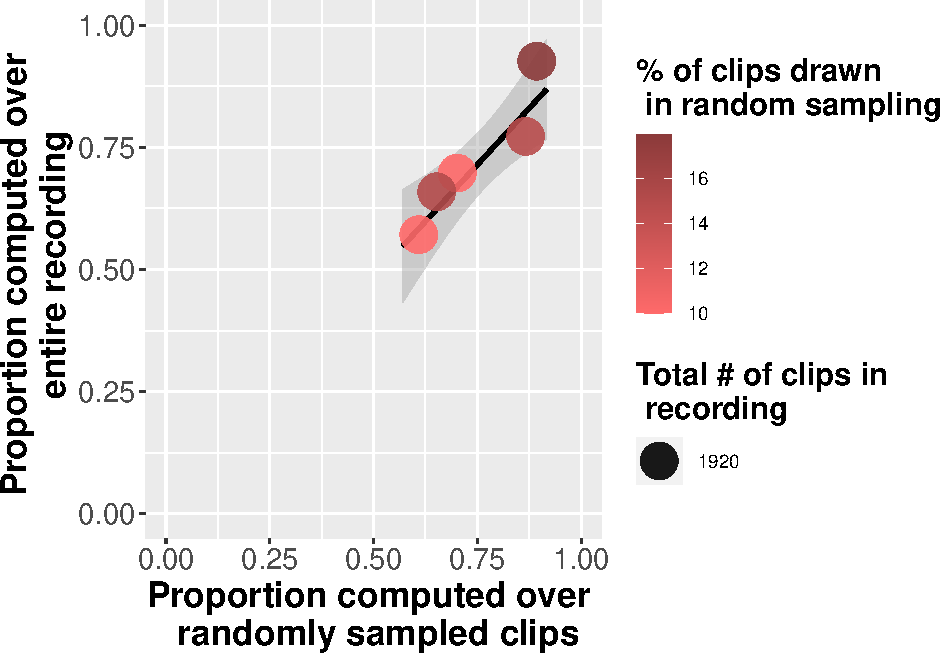
\includegraphics{validation_results_files/figure-latex/us plot-1.pdf}

\begin{Shaded}
\begin{Highlighting}[]
\KeywordTok{jpeg}\NormalTok{(}\StringTok{"/Users/megcychosz/Google Drive/biling_CDS/results/figures/us_plot.jpeg"}\NormalTok{, }\DataTypeTok{height =} \DecValTok{500}\NormalTok{, }\DataTypeTok{width =} \DecValTok{600}\NormalTok{)}
\NormalTok{us_plot}
\KeywordTok{dev.off}\NormalTok{()}
\end{Highlighting}
\end{Shaded}

\begin{verbatim}
## pdf 
##   2
\end{verbatim}

\begin{Shaded}
\begin{Highlighting}[]
\NormalTok{bo_plot <-}\StringTok{ }\NormalTok{plot_data }\OperatorTok
\StringTok{  }\KeywordTok{filter}\NormalTok{(location}\OperatorTok{==}\StringTok{'Bolivia'}\NormalTok{) }\OperatorTok
\StringTok{  }\KeywordTok{distinct_at}\NormalTok{(., }\KeywordTok{vars}\NormalTok{(method, id), }\DataTypeTok{.keep_all =}\NormalTok{ T) }\OperatorTok
\StringTok{  }\KeywordTok{select}\NormalTok{(}\OperatorTok{-}\NormalTok{percen_span, }\OperatorTok{-}\NormalTok{percen_ofallclips_drawn, }\OperatorTok{-}\NormalTok{percen_mxd, }\OperatorTok{-}\NormalTok{speech_clips, }\OperatorTok{-}\NormalTok{total) }\OperatorTok
\StringTok{  }\KeywordTok{spread}\NormalTok{(}\StringTok{"method"}\NormalTok{, }\StringTok{"percen_que"}\NormalTok{) }\OperatorTok
\StringTok{  }\KeywordTok{merge}\NormalTok{(., per_ann, }\DataTypeTok{by=}\StringTok{'id'}\NormalTok{) }\OperatorTok
\StringTok{  }\KeywordTok{distinct}\NormalTok{(id, }\DataTypeTok{.keep_all =}\NormalTok{ T) }\OperatorTok
\KeywordTok{ggplot}\NormalTok{(., }\KeywordTok{aes}\NormalTok{(random, complete)) }\OperatorTok{+}
\StringTok{  }\KeywordTok{geom_smooth}\NormalTok{(}\DataTypeTok{method =} \StringTok{"lm"}\NormalTok{, }\DataTypeTok{color=}\StringTok{"black"}\NormalTok{) }\OperatorTok{+}
\StringTok{  }\KeywordTok{geom_jitter}\NormalTok{(}\KeywordTok{aes}\NormalTok{(}\DataTypeTok{size=}\NormalTok{num_clips,}\DataTypeTok{color=}\KeywordTok{round}\NormalTok{(percen_ofallclips_drawn,}\DecValTok{2}\NormalTok{)),}\DataTypeTok{alpha=}\NormalTok{.}\DecValTok{9}\NormalTok{,}\DataTypeTok{position =} \KeywordTok{position_jitter}\NormalTok{(}\DataTypeTok{width =} \FloatTok{0.07}\NormalTok{, }\DataTypeTok{height =} \FloatTok{.01}\NormalTok{)) }\OperatorTok{+}
\StringTok{  }\KeywordTok{scale_size_continuous}\NormalTok{(}\DataTypeTok{range =} \KeywordTok{c}\NormalTok{(}\DecValTok{5}\NormalTok{, }\DecValTok{9}\NormalTok{)) }\OperatorTok{+}\StringTok{ }
\StringTok{  }\KeywordTok{scale_colour_gradient}\NormalTok{(}\DataTypeTok{low=}\StringTok{'indianred1'}\NormalTok{, }\DataTypeTok{high =} \StringTok{'indianred4'}\NormalTok{) }\OperatorTok{+}
\StringTok{  }\KeywordTok{ylab}\NormalTok{(}\StringTok{"Proportion computed over }\CharTok{\textbackslash{}n}\StringTok{ entire recording"}\NormalTok{) }\OperatorTok{+}\StringTok{ }
\StringTok{  }\KeywordTok{xlab}\NormalTok{(}\StringTok{"Proportion computed over }\CharTok{\textbackslash{}n}\StringTok{ randomly sampled clips"}\NormalTok{) }\OperatorTok{+}\StringTok{ }
\StringTok{  }\KeywordTok{ylim}\NormalTok{(}\DecValTok{0}\NormalTok{,}\DecValTok{1}\NormalTok{) }\OperatorTok{+}
\StringTok{  }\KeywordTok{xlim}\NormalTok{(}\DecValTok{0}\NormalTok{,}\DecValTok{1}\NormalTok{)}\OperatorTok{+}
\StringTok{  }\CommentTok{#facet_wrap(~location, scales = "free") +}
\StringTok{  }\KeywordTok{labs}\NormalTok{(}\DataTypeTok{col=}\StringTok{'% of clips drawn }\CharTok{\textbackslash{}n}\StringTok{ in random sampling'}\NormalTok{) }\OperatorTok{+}\StringTok{ }
\StringTok{       }\CommentTok{#title = 'Proportion of Quechua clips \textbackslash{}n in Bolivian corpus') +}
\StringTok{ }\KeywordTok{theme}\NormalTok{(}\DataTypeTok{title =} \KeywordTok{element_text}\NormalTok{(}\DataTypeTok{size=}\DecValTok{18}\NormalTok{, }\DataTypeTok{face=}\StringTok{"bold"}\NormalTok{),}
   \DataTypeTok{axis.text=}\KeywordTok{element_text}\NormalTok{(}\DataTypeTok{size=}\DecValTok{14}\NormalTok{),}
      \DataTypeTok{axis.title=}\KeywordTok{element_text}\NormalTok{(}\DataTypeTok{size=}\DecValTok{17}\NormalTok{,}\DataTypeTok{face=}\StringTok{"bold"}\NormalTok{),}
      \DataTypeTok{legend.title =} \KeywordTok{element_text}\NormalTok{(}\DataTypeTok{size=}\DecValTok{15}\NormalTok{))}\OperatorTok{+}
\StringTok{       }\CommentTok{#legend.position = c(.8, .5)) +}
\StringTok{      }\KeywordTok{guides}\NormalTok{(}\DataTypeTok{size=}\KeywordTok{guide_legend}\NormalTok{(}\DataTypeTok{title=}\StringTok{"Total # of clips in }\CharTok{\textbackslash{}n}\StringTok{ recording"}\NormalTok{))}
\NormalTok{bo_plot}
\end{Highlighting}
\end{Shaded}

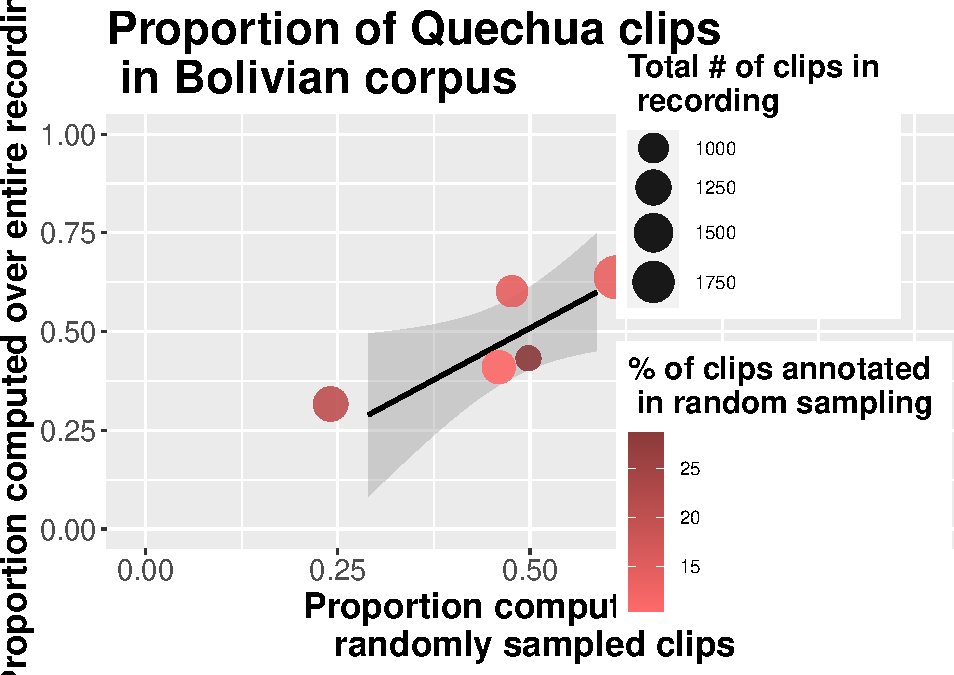
\includegraphics{validation_results_files/figure-latex/bolivia plot-1.pdf}

\begin{Shaded}
\begin{Highlighting}[]
\KeywordTok{jpeg}\NormalTok{(}\StringTok{"/Users/megcychosz/Google Drive/biling_CDS/results/figures/bolivia_plot.jpeg"}\NormalTok{, }\DataTypeTok{height =} \DecValTok{500}\NormalTok{, }\DataTypeTok{width =} \DecValTok{600}\NormalTok{)}
\NormalTok{bo_plot}
\KeywordTok{dev.off}\NormalTok{()}
\end{Highlighting}
\end{Shaded}

\begin{verbatim}
## pdf 
##   2
\end{verbatim}

\hypertarget{chid-directed-speech-across-random-and-full-methods}{%
\subsubsection{Chid-directed speech across random and full methods}\label{chid-directed-speech-across-random-and-full-methods}}

\begin{Shaded}
\begin{Highlighting}[]
\NormalTok{reg_annon <-}\StringTok{ }\NormalTok{data_annon }\OperatorTok
\StringTok{  }\KeywordTok{filter}\NormalTok{(addressee}\OperatorTok{==}\StringTok{'Adult2TargetChild'} \OperatorTok{|}\StringTok{ }\NormalTok{addressee}\OperatorTok{==}\StringTok{'Otherchild2TargetChild'} \OperatorTok{|}\StringTok{ }\NormalTok{addressee}\OperatorTok{==}\StringTok{'Adult2Others'} \OperatorTok{|}\StringTok{ }\NormalTok{addressee}\OperatorTok{==}\StringTok{'Otherchild2adults'} \OperatorTok{|}\StringTok{ }\NormalTok{addressee}\OperatorTok{==}\StringTok{'Adult2OtherChild'} \OperatorTok{|}\StringTok{ }\NormalTok{addressee}\OperatorTok{==}\StringTok{'Otherchild2OtherChild'}\NormalTok{) }\OperatorTok\StringTok{ }\CommentTok{# only clips where we know the register}
\StringTok{  }\KeywordTok{group_by}\NormalTok{(id, method) }\OperatorTok
\StringTok{  }\KeywordTok{distinct_at}\NormalTok{(., }\KeywordTok{vars}\NormalTok{(file_name, addressee), }\DataTypeTok{.keep_all =}\NormalTok{ T) }\OperatorTok\StringTok{ }\CommentTok{# don't record multiple speakers speaking the same register}
\StringTok{  }\KeywordTok{mutate}\NormalTok{(}\DataTypeTok{total_reg_annotations =} \KeywordTok{NROW}\NormalTok{(file_name))}\CommentTok{# N of register annotations made; distinct from N of speech clips since one clip could contain multiple registers; distinct from total_annotations because this measure doesn't include 'unsure'}

\NormalTok{cds <-}\StringTok{ }\NormalTok{reg_annon }\OperatorTok\StringTok{ }
\StringTok{  }\KeywordTok{group_by}\NormalTok{(id, method) }\OperatorTok
\StringTok{  }\KeywordTok{filter}\NormalTok{(addressee}\OperatorTok{==}\StringTok{'Adult2TargetChild'} \OperatorTok{|}\StringTok{ }\NormalTok{addressee}\OperatorTok{==}\StringTok{'Otherchild2TargetChild'}\NormalTok{) }\OperatorTok
\StringTok{  }\KeywordTok{group_by}\NormalTok{(method) }\OperatorTok
\StringTok{  }\KeywordTok{distinct}\NormalTok{(file_name, }\DataTypeTok{.keep_all =}\NormalTok{ T) }\OperatorTok\StringTok{ }
\StringTok{  }\KeywordTok{group_by}\NormalTok{(id, method) }\OperatorTok
\StringTok{  }\KeywordTok{mutate}\NormalTok{(}\DataTypeTok{n_cds =} \KeywordTok{n}\NormalTok{()) }\OperatorTok\StringTok{ }\CommentTok{# # of CDS clips }
\StringTok{  }\KeywordTok{distinct_at}\NormalTok{(., }\KeywordTok{vars}\NormalTok{(id, method), }\DataTypeTok{.keep_all =}\NormalTok{ T) }\OperatorTok
\StringTok{  }\KeywordTok{mutate}\NormalTok{(}\DataTypeTok{percen_cds =}\NormalTok{ n_cds }\OperatorTok{/}\StringTok{ }\NormalTok{total_reg_annotations) }\OperatorTok
\StringTok{  }\KeywordTok{select}\NormalTok{(id, num_clips, age_YYMMDD, gender, location, method, percen_cds, n_cds, percen_ofallclips_drawn)}

\NormalTok{ads <-}\StringTok{ }\NormalTok{reg_annon }\OperatorTok\StringTok{ }
\StringTok{  }\KeywordTok{filter}\NormalTok{(addressee}\OperatorTok{==}\StringTok{'Adult2Others'} \OperatorTok{|}\StringTok{ }\NormalTok{addressee}\OperatorTok{==}\StringTok{'Otherchild2adults'}\NormalTok{) }\OperatorTok
\StringTok{  }\KeywordTok{group_by}\NormalTok{(method) }\OperatorTok\StringTok{ }
\StringTok{  }\KeywordTok{distinct}\NormalTok{(file_name, }\DataTypeTok{.keep_all =}\NormalTok{ T) }\OperatorTok\StringTok{ }
\StringTok{  }\KeywordTok{group_by}\NormalTok{(id, method) }\OperatorTok\StringTok{  }
\StringTok{  }\KeywordTok{mutate}\NormalTok{(}\DataTypeTok{n_ads =} \KeywordTok{n}\NormalTok{()) }\OperatorTok\StringTok{ }\CommentTok{# # of ADS clips}
\StringTok{  }\KeywordTok{distinct_at}\NormalTok{(., }\KeywordTok{vars}\NormalTok{(id, method), }\DataTypeTok{.keep_all =}\NormalTok{ T) }\OperatorTok
\StringTok{  }\KeywordTok{mutate}\NormalTok{(}\DataTypeTok{percen_ads =}\NormalTok{ n_ads }\OperatorTok{/}\StringTok{ }\NormalTok{total_reg_annotations) }\OperatorTok
\StringTok{  }\KeywordTok{select}\NormalTok{(id, num_clips, age_YYMMDD, gender, location, method, percen_ads, n_ads, percen_ofallclips_drawn)}

\NormalTok{o_child <-}\StringTok{ }\NormalTok{reg_annon }\OperatorTok\StringTok{ }
\StringTok{  }\KeywordTok{filter}\NormalTok{(addressee}\OperatorTok{==}\StringTok{'Adult2OtherChild'} \OperatorTok{|}\StringTok{ }\NormalTok{addressee}\OperatorTok{==}\StringTok{'Otherchild2OtherChild'}\NormalTok{) }\OperatorTok
\StringTok{  }\KeywordTok{group_by}\NormalTok{(method) }\OperatorTok\StringTok{ }
\StringTok{  }\KeywordTok{distinct}\NormalTok{(file_name, }\DataTypeTok{.keep_all =}\NormalTok{ T) }\OperatorTok\StringTok{ }
\StringTok{  }\KeywordTok{group_by}\NormalTok{(id, method) }\OperatorTok\StringTok{  }
\StringTok{  }\KeywordTok{mutate}\NormalTok{(}\DataTypeTok{n_ods =} \KeywordTok{n}\NormalTok{()) }\OperatorTok\StringTok{ }\CommentTok{# # of ODS clips}
\StringTok{  }\KeywordTok{distinct_at}\NormalTok{(., }\KeywordTok{vars}\NormalTok{(id, method), }\DataTypeTok{.keep_all =}\NormalTok{ T) }\OperatorTok
\StringTok{  }\KeywordTok{mutate}\NormalTok{(}\DataTypeTok{percen_ods =}\NormalTok{ n_ods }\OperatorTok{/}\StringTok{ }\NormalTok{total_reg_annotations) }\OperatorTok
\StringTok{  }\KeywordTok{select}\NormalTok{(id, num_clips, age_YYMMDD, gender, location, method, percen_ods, n_ods, percen_ofallclips_drawn)}

\NormalTok{o2 <-}\StringTok{ }\KeywordTok{merge}\NormalTok{(cds, ads, }\DataTypeTok{all=}\NormalTok{T)}
\NormalTok{o3 <-}\StringTok{ }\KeywordTok{merge}\NormalTok{(o2, o_child, }\DataTypeTok{all =}\NormalTok{ T)}
\NormalTok{o3[}\KeywordTok{is.na}\NormalTok{(o3)] <-}\StringTok{ }\DecValTok{0} \CommentTok{# one child doesn't have any ODS}

\CommentTok{# sanity check}
\NormalTok{o3}\OperatorTok{$}\NormalTok{total <-}\StringTok{ }\NormalTok{o3}\OperatorTok{$}\NormalTok{percen_ods }\OperatorTok{+}\StringTok{ }\NormalTok{o3}\OperatorTok{$}\NormalTok{percen_ads }\OperatorTok{+}\StringTok{ }\NormalTok{o3}\OperatorTok{$}\NormalTok{percen_cds}
\end{Highlighting}
\end{Shaded}

\begin{Shaded}
\begin{Highlighting}[]
\CommentTok{# for later}
\NormalTok{percen_cds_df <-}\StringTok{ }\NormalTok{o3 }\OperatorTok
\StringTok{  }\KeywordTok{distinct_at}\NormalTok{(., }\KeywordTok{vars}\NormalTok{(id, method), }\DataTypeTok{.keep_all =}\NormalTok{ T) }\OperatorTok
\StringTok{  }\KeywordTok{filter}\NormalTok{(method}\OperatorTok{==}\StringTok{'random'}\NormalTok{) }\OperatorTok
\StringTok{  }\KeywordTok{select}\NormalTok{(id, percen_ofallclips_drawn) }\CommentTok{# get the % of clips annotated for each id and method}

\NormalTok{cds_plot_data <-}\StringTok{ }\NormalTok{o3 }\OperatorTok
\StringTok{  }\KeywordTok{select}\NormalTok{(id, gender, location, num_clips, method, percen_cds) }\OperatorTok
\StringTok{  }\KeywordTok{spread}\NormalTok{(}\StringTok{"method"}\NormalTok{, }\StringTok{"percen_cds"}\NormalTok{) }\OperatorTok
\StringTok{  }\KeywordTok{merge}\NormalTok{(., percen_cds_df, }\DataTypeTok{by=}\StringTok{'id'}\NormalTok{)}

\CommentTok{# compute correlations}
\NormalTok{cds_cors <-}\StringTok{ }\NormalTok{cds_plot_data }\OperatorTok
\StringTok{  }\KeywordTok{group_by}\NormalTok{(location) }\OperatorTok
\StringTok{  }\KeywordTok{summarize}\NormalTok{(., }\KeywordTok{paste}\NormalTok{(}\StringTok{"r="}\NormalTok{,}\KeywordTok{round}\NormalTok{(}\KeywordTok{cor.test}\NormalTok{(complete, random)}\OperatorTok{$}\NormalTok{estimate,}\DecValTok{2}\NormalTok{),}\StringTok{","}\NormalTok{,}\StringTok{"p="}\NormalTok{,}\KeywordTok{round}\NormalTok{(}\KeywordTok{cor.test}\NormalTok{(complete, random)}\OperatorTok{$}\NormalTok{p.value,}\DecValTok{2}\NormalTok{)))}

\CommentTok{#reg_tbl <- o3 %>%}
\CommentTok{#  group_by(method, location) %>%}
\CommentTok{#  summarize(avg=round(mean(percen_cds),2),}
\CommentTok{#            sd=round(sd(percen_cds),2)) %>%}
\CommentTok{#  mutate(stats=paste(avg,"(",sd,")")) %>%}
\CommentTok{#  select(-avg, -sd) %>%}
\CommentTok{#  spread(key='method', value = "stats") }

\CommentTok{# calculate relative errors}
\NormalTok{cds_rel_error <-}\StringTok{ }\NormalTok{o3 }\OperatorTok
\StringTok{  }\KeywordTok{group_by}\NormalTok{(id) }\OperatorTok
\StringTok{  }\CommentTok{#summarize(avg=mean(percen_cds)) %>%}
\StringTok{  }\KeywordTok{select}\NormalTok{(id,method,percen_cds,location) }\OperatorTok
\StringTok{  }\KeywordTok{spread}\NormalTok{(}\DataTypeTok{key=}\StringTok{'method'}\NormalTok{, }\DataTypeTok{value=}\StringTok{'percen_cds'}\NormalTok{) }\OperatorTok
\StringTok{  }\KeywordTok{mutate}\NormalTok{(}\DataTypeTok{relative_error =} \KeywordTok{round}\NormalTok{(((}\KeywordTok{abs}\NormalTok{(random }\OperatorTok{-}\StringTok{ }\NormalTok{complete) }\OperatorTok{/}\StringTok{ }\NormalTok{complete)}\OperatorTok{*}\DecValTok{100}\NormalTok{),}\DecValTok{2}\NormalTok{)) }\OperatorTok
\StringTok{  }\CommentTok{#mutate(avg_rel_error = round(mean(relative_error),2),}
\StringTok{  }\CommentTok{#       sd_rel_error = round(sd(relative_error),2),}
\StringTok{  }\CommentTok{#       rel_error_stats=paste(avg_rel_error,"(",sd_rel_error,")")) %>%}
\StringTok{  }\KeywordTok{distinct}\NormalTok{(relative_error, }\DataTypeTok{.keep_all =}\NormalTok{ T)}




\CommentTok{# add correlations to table - will make pretty below}
\NormalTok{final_reg_tbl <-}\StringTok{ }\KeywordTok{merge}\NormalTok{(cds_rel_error, cds_cors, }\DataTypeTok{by=}\StringTok{'location'}\NormalTok{)}

\NormalTok{final_reg_tbl}\OperatorTok{$}\NormalTok{location <-}\StringTok{ }
\StringTok{  }\NormalTok{plyr}\OperatorTok{::}\KeywordTok{mapvalues}\NormalTok{(final_reg_tbl}\OperatorTok{$}\NormalTok{location, }
                  \DataTypeTok{from =} \KeywordTok{c}\NormalTok{(}\StringTok{"Bolivia"}\NormalTok{, }\StringTok{"US"}\NormalTok{), }
                  \DataTypeTok{to =}\KeywordTok{c}\NormalTok{(}\StringTok{"Quechua-Spanish"}\NormalTok{, }\StringTok{"Spanish-English"}\NormalTok{))}

\NormalTok{final_reg_tbl2 <-}\StringTok{ }\NormalTok{final_reg_tbl }\OperatorTok
\StringTok{  }\KeywordTok{mutate}\NormalTok{(}\DataTypeTok{random =} \KeywordTok{round}\NormalTok{(random,}\DecValTok{2}\NormalTok{),}
         \DataTypeTok{complete =} \KeywordTok{round}\NormalTok{(complete,}\DecValTok{2}\NormalTok{)) }\OperatorTok
\StringTok{  }\KeywordTok{mutate}\NormalTok{(}\DataTypeTok{corpus_id =} \KeywordTok{paste}\NormalTok{(location,}\StringTok{"("}\NormalTok{,id,}\StringTok{")"}\NormalTok{)) }\OperatorTok
\StringTok{  }\KeywordTok{select}\NormalTok{(}\OperatorTok{-}\NormalTok{location, }\OperatorTok{-}\NormalTok{id) }\OperatorTok
\StringTok{  }\KeywordTok{relocate}\NormalTok{(corpus_id, random, complete)}
  


\NormalTok{knitr}\OperatorTok{::}\KeywordTok{kable}\NormalTok{(final_reg_tbl2, }\DataTypeTok{caption =} \StringTok{'Child-directed speech estimates by child and annotation method.'}\NormalTok{, }
             \DataTypeTok{booktabs=}\NormalTok{T, }
             \DataTypeTok{row.names =} \OtherTok{FALSE}\NormalTok{, }
             \DataTypeTok{col.names =} \KeywordTok{c}\NormalTok{(}\StringTok{"Corpus (ID)"}\NormalTok{, }\StringTok{"Random"}\NormalTok{, }\StringTok{"All-day"}\NormalTok{, }\StringTok{"Relative error"}\NormalTok{, }\StringTok{"Within-corpus correlation between estimates"}\NormalTok{)) }\OperatorTok\StringTok{ }\CommentTok{# "}
\StringTok{  }\CommentTok{#column_spec(2, width = "4cm") %>% # force column headers onto two rows}
\StringTok{  }\CommentTok{#column_spec(3, width = "3cm") %>%}
\StringTok{  }\KeywordTok{column_spec}\NormalTok{(}\DecValTok{5}\NormalTok{, }\DataTypeTok{width =} \StringTok{"5cm"}\NormalTok{) }\OperatorTok
\StringTok{  }\KeywordTok{kable_styling}\NormalTok{() }\OperatorTok
\StringTok{  }\KeywordTok{add_header_above}\NormalTok{(}\KeywordTok{c}\NormalTok{(}\StringTok{" "}\NormalTok{ =}\StringTok{ }\DecValTok{1}\NormalTok{, }\StringTok{"Annotation Method"}\NormalTok{ =}\StringTok{ }\DecValTok{2}\NormalTok{, }\StringTok{" "}\NormalTok{ =}\StringTok{ }\DecValTok{2}\NormalTok{)) }\OperatorTok
\StringTok{  }\NormalTok{kableExtra}\OperatorTok{::}\KeywordTok{kable_styling}\NormalTok{(}\DataTypeTok{latex_options =} \StringTok{"hold_position"}\NormalTok{)}
\end{Highlighting}
\end{Shaded}

\begin{table}[!h]

\caption{(\#tab:cds proportion stats)Child-directed speech estimates by child and annotation method.}
\centering
\begin{tabular}[t]{lrrr>{\raggedright\arraybackslash}p{5cm}}
\toprule
\multicolumn{1}{c}{ } & \multicolumn{2}{c}{Annotation Method} & \multicolumn{2}{c}{ } \\
\cmidrule(l{3pt}r{3pt}){2-3}
Corpus (ID) & Random & All-day & Relative error & Within-corpus correlation between estimates\\
\midrule
Quechua-Spanish ( 1032 ) & 0.18 & 0.17 & 5.95 & r= 0.63 , p= 0.26\\
Quechua-Spanish ( 1060 ) & 0.12 & 0.07 & 55.09 & r= 0.63 , p= 0.26\\
Quechua-Spanish ( 1075 ) & 0.12 & 0.14 & 12.50 & r= 0.63 , p= 0.26\\
Quechua-Spanish ( 1077 ) & 0.10 & 0.11 & 10.48 & r= 0.63 , p= 0.26\\
Quechua-Spanish ( 1081 ) & 0.13 & 0.05 & 145.09 & r= 0.63 , p= 0.26\\
\addlinespace
Spanish-English ( 179 ) & 0.52 & 0.46 & 12.61 & r= 0.97 , p= 0.01\\
Spanish-English ( 198-9mo ) & 0.65 & 0.66 & 0.54 & r= 0.97 , p= 0.01\\
Spanish-English ( 199 ) & 0.28 & 0.30 & 6.24 & r= 0.97 , p= 0.01\\
Spanish-English ( 261-8mo ) & 0.77 & 0.79 & 2.32 & r= 0.97 , p= 0.01\\
Spanish-English ( 267-12mo ) & 0.40 & 0.47 & 15.23 & r= 0.97 , p= 0.01\\
\bottomrule
\end{tabular}
\end{table}

\begin{Shaded}
\begin{Highlighting}[]
\NormalTok{ads_plot_data <-}\StringTok{ }\NormalTok{o3 }\OperatorTok
\StringTok{  }\CommentTok{#filter(location=='Bolivia') %>%}
\StringTok{  }\KeywordTok{select}\NormalTok{(id, gender, location, num_clips, method, percen_ads) }\OperatorTok
\StringTok{  }\KeywordTok{spread}\NormalTok{(}\StringTok{"method"}\NormalTok{, }\StringTok{"percen_ads"}\NormalTok{) }\OperatorTok
\StringTok{  }\KeywordTok{merge}\NormalTok{(., percen_cds_df, }\DataTypeTok{by=}\StringTok{'id'}\NormalTok{)}

\CommentTok{# compute correlations}
\NormalTok{ads_cors <-}\StringTok{ }\NormalTok{ads_plot_data }\OperatorTok
\StringTok{  }\KeywordTok{group_by}\NormalTok{(location) }\OperatorTok
\StringTok{  }\KeywordTok{summarize}\NormalTok{(., }\KeywordTok{paste}\NormalTok{(}\StringTok{"r="}\NormalTok{,}\KeywordTok{round}\NormalTok{(}\KeywordTok{cor.test}\NormalTok{(complete, random)}\OperatorTok{$}\NormalTok{estimate,}\DecValTok{2}\NormalTok{),}\StringTok{","}\NormalTok{,}\StringTok{"p="}\NormalTok{,}\KeywordTok{round}\NormalTok{(}\KeywordTok{cor.test}\NormalTok{(complete, random)}\OperatorTok{$}\NormalTok{p.value,}\DecValTok{2}\NormalTok{)))}

\NormalTok{reg_tbl <-}\StringTok{ }\NormalTok{o3 }\OperatorTok
\StringTok{  }\KeywordTok{group_by}\NormalTok{(method, location) }\OperatorTok
\StringTok{  }\KeywordTok{summarize}\NormalTok{(}\DataTypeTok{avg=}\KeywordTok{round}\NormalTok{(}\KeywordTok{mean}\NormalTok{(percen_ads),}\DecValTok{2}\NormalTok{),}
            \DataTypeTok{sd=}\KeywordTok{round}\NormalTok{(}\KeywordTok{sd}\NormalTok{(percen_ads),}\DecValTok{2}\NormalTok{)) }\OperatorTok
\StringTok{  }\KeywordTok{mutate}\NormalTok{(}\DataTypeTok{stats=}\KeywordTok{paste}\NormalTok{(avg,}\StringTok{"("}\NormalTok{,sd,}\StringTok{")"}\NormalTok{)) }\OperatorTok
\StringTok{  }\KeywordTok{select}\NormalTok{(}\OperatorTok{-}\NormalTok{avg, }\OperatorTok{-}\NormalTok{sd) }\OperatorTok
\StringTok{  }\KeywordTok{spread}\NormalTok{(}\DataTypeTok{key=}\StringTok{'method'}\NormalTok{, }\DataTypeTok{value =} \StringTok{"stats"}\NormalTok{) }

\CommentTok{# calculate relative errors}
\NormalTok{ads_rel_error <-}\StringTok{ }\NormalTok{o3 }\OperatorTok
\StringTok{  }\KeywordTok{group_by}\NormalTok{(method, location, id) }\OperatorTok
\StringTok{  }\KeywordTok{summarize}\NormalTok{(}\DataTypeTok{avg=}\KeywordTok{mean}\NormalTok{(percen_ads)) }\OperatorTok
\StringTok{  }\KeywordTok{spread}\NormalTok{(}\DataTypeTok{key=}\StringTok{'method'}\NormalTok{, }\DataTypeTok{value=}\StringTok{'avg'}\NormalTok{) }\OperatorTok
\StringTok{  }\KeywordTok{group_by}\NormalTok{(id) }\OperatorTok
\StringTok{  }\KeywordTok{mutate}\NormalTok{(}\DataTypeTok{relative_error =}\NormalTok{ ((}\KeywordTok{abs}\NormalTok{(random }\OperatorTok{-}\StringTok{ }\NormalTok{complete) }\OperatorTok{/}\StringTok{ }\NormalTok{complete)}\OperatorTok{*}\DecValTok{100}\NormalTok{)) }\OperatorTok
\StringTok{  }\KeywordTok{ungroup}\NormalTok{() }\OperatorTok
\StringTok{  }\KeywordTok{group_by}\NormalTok{(location) }\OperatorTok
\StringTok{  }\KeywordTok{mutate}\NormalTok{(}\DataTypeTok{avg_rel_error =} \KeywordTok{round}\NormalTok{(}\KeywordTok{mean}\NormalTok{(relative_error),}\DecValTok{2}\NormalTok{),}
         \DataTypeTok{sd_rel_error =} \KeywordTok{round}\NormalTok{(}\KeywordTok{sd}\NormalTok{(relative_error),}\DecValTok{2}\NormalTok{),}
         \DataTypeTok{rel_error_stats=}\KeywordTok{paste}\NormalTok{(avg_rel_error,}\StringTok{"("}\NormalTok{,sd_rel_error,}\StringTok{")"}\NormalTok{)) }\OperatorTok
\StringTok{  }\KeywordTok{distinct}\NormalTok{(rel_error_stats)}

\CommentTok{# add correlations to table - will make pretty below}
\NormalTok{final_reg_tbl <-}\StringTok{ }\KeywordTok{merge}\NormalTok{(reg_tbl, ads_cors, }\DataTypeTok{by=}\StringTok{'location'}\NormalTok{)}
\NormalTok{final_reg_tbl2 <-}\StringTok{ }\KeywordTok{merge}\NormalTok{(final_reg_tbl, ads_rel_error, }\DataTypeTok{by=}\StringTok{'location'}\NormalTok{)}
\NormalTok{final_reg_tbl}\OperatorTok{$}\NormalTok{location <-}\StringTok{ }
\StringTok{  }\NormalTok{plyr}\OperatorTok{::}\KeywordTok{mapvalues}\NormalTok{(final_reg_tbl}\OperatorTok{$}\NormalTok{location, }
                  \DataTypeTok{from =} \KeywordTok{c}\NormalTok{(}\StringTok{"Bolivia"}\NormalTok{, }\StringTok{"US"}\NormalTok{), }
                  \DataTypeTok{to =}\KeywordTok{c}\NormalTok{(}\StringTok{"Quechua-Spanish"}\NormalTok{, }\StringTok{"Spanish-English"}\NormalTok{))}

\NormalTok{knitr}\OperatorTok{::}\KeywordTok{kable}\NormalTok{(final_reg_tbl2, }\DataTypeTok{caption =} \StringTok{'Average adult-directed speech estimates by corpus and annotation method.'}\NormalTok{, }
             \DataTypeTok{booktabs=}\NormalTok{T, }
             \DataTypeTok{row.names =} \OtherTok{FALSE}\NormalTok{, }
             \DataTypeTok{col.names =} \KeywordTok{c}\NormalTok{(}\StringTok{"Corpus"}\NormalTok{, }\StringTok{"Random"}\NormalTok{, }\StringTok{"All-day"}\NormalTok{, }\StringTok{"Correlation between estimates"}\NormalTok{, }\StringTok{"Average relative error (SD)"}\NormalTok{)) }\OperatorTok\StringTok{ }
\StringTok{  }\KeywordTok{kable_styling}\NormalTok{() }\OperatorTok
\StringTok{  }\KeywordTok{add_header_above}\NormalTok{(}\KeywordTok{c}\NormalTok{(}\StringTok{" "}\NormalTok{ =}\StringTok{ }\DecValTok{1}\NormalTok{, }\StringTok{"Annotation Method"}\NormalTok{ =}\StringTok{ }\DecValTok{2}\NormalTok{, }\StringTok{" "}\NormalTok{ =}\StringTok{ }\DecValTok{2}\NormalTok{)) }\OperatorTok
\StringTok{  }\NormalTok{kableExtra}\OperatorTok{::}\KeywordTok{kable_styling}\NormalTok{(}\DataTypeTok{latex_options =} \StringTok{"hold_position"}\NormalTok{)}
\end{Highlighting}
\end{Shaded}

\begin{table}[!h]

\caption{(\#tab:ads proportion stats)Average adult-directed speech estimates by corpus and annotation method.}
\centering
\begin{tabular}[t]{lllll}
\toprule
\multicolumn{1}{c}{ } & \multicolumn{2}{c}{Annotation Method} & \multicolumn{2}{c}{ } \\
\cmidrule(l{3pt}r{3pt}){2-3}
Corpus & Random & All-day & Correlation between estimates & Average relative error (SD)\\
\midrule
Bolivia & 0.45 ( 0.13 ) & 0.4 ( 0.09 ) & r= 0.84 , p= 0.07 & 11.56 ( 12.11 )\\
US & 0.27 ( 0.17 ) & 0.27 ( 0.2 ) & r= 0.96 , p= 0.01 & 16.75 ( 12.45 )\\
\bottomrule
\end{tabular}
\end{table}

\begin{Shaded}
\begin{Highlighting}[]
\CommentTok{# reorder location variable}
\NormalTok{cds_plot_data}\OperatorTok{$}\NormalTok{location <-}\StringTok{ }\KeywordTok{factor}\NormalTok{(cds_plot_data}\OperatorTok{$}\NormalTok{location, }\DataTypeTok{levels =} \KeywordTok{c}\NormalTok{(}\StringTok{"US"}\NormalTok{, }\StringTok{"Bolivia"}\NormalTok{))}

\NormalTok{cds_plot <-}\StringTok{ }\KeywordTok{ggplot}\NormalTok{(cds_plot_data, }\KeywordTok{aes}\NormalTok{(random, complete)) }\OperatorTok{+}
\StringTok{  }\KeywordTok{geom_smooth}\NormalTok{(}\DataTypeTok{method =} \StringTok{"lm"}\NormalTok{, }\DataTypeTok{color=}\StringTok{"black"}\NormalTok{) }\OperatorTok{+}
\StringTok{  }\KeywordTok{geom_jitter}\NormalTok{(}\KeywordTok{aes}\NormalTok{(}\DataTypeTok{size=}\NormalTok{num_clips,}\DataTypeTok{color=}\KeywordTok{round}\NormalTok{(percen_ofallclips_drawn,}\DecValTok{2}\NormalTok{)),}\DataTypeTok{alpha=}\NormalTok{.}\DecValTok{9}\NormalTok{,}\DataTypeTok{position =} \KeywordTok{position_jitter}\NormalTok{(}\DataTypeTok{width =} \FloatTok{0.07}\NormalTok{, }\DataTypeTok{height =} \FloatTok{.01}\NormalTok{)) }\OperatorTok{+}
\StringTok{  }\KeywordTok{scale_size_continuous}\NormalTok{(}\DataTypeTok{range =} \KeywordTok{c}\NormalTok{(}\DecValTok{5}\NormalTok{, }\DecValTok{9}\NormalTok{)) }\OperatorTok{+}\StringTok{ }
\StringTok{  }\KeywordTok{scale_colour_gradient}\NormalTok{(}\DataTypeTok{low=}\StringTok{'indianred1'}\NormalTok{, }\DataTypeTok{high =} \StringTok{'indianred4'}\NormalTok{) }\OperatorTok{+}
\StringTok{  }\KeywordTok{ylab}\NormalTok{(}\StringTok{"Proportion computed over entire recording"}\NormalTok{) }\OperatorTok{+}\StringTok{ }
\StringTok{  }\KeywordTok{xlab}\NormalTok{(}\StringTok{"Proportion computed over randomly sampled clips"}\NormalTok{) }\OperatorTok{+}\StringTok{ }
\StringTok{  }\KeywordTok{ylim}\NormalTok{(}\DecValTok{0}\NormalTok{,}\FloatTok{0.9}\NormalTok{) }\OperatorTok{+}
\StringTok{  }\KeywordTok{xlim}\NormalTok{(}\DecValTok{0}\NormalTok{,}\FloatTok{0.9}\NormalTok{)}\OperatorTok{+}
\StringTok{  }\KeywordTok{facet_wrap}\NormalTok{(}\OperatorTok{~}\NormalTok{location, }\DataTypeTok{scales =} \StringTok{"fixed"}\NormalTok{) }\OperatorTok{+}
\StringTok{  }\KeywordTok{labs}\NormalTok{(}\DataTypeTok{col=}\StringTok{'% of clips annotated }\CharTok{\textbackslash{}n}\StringTok{ in random sampling'}\NormalTok{) }\OperatorTok{+}\StringTok{ }
\StringTok{       }\CommentTok{#title = 'Proportion of child-directed speech clips \textbackslash{}n in U.S. and Bolivian corpora') +}
\StringTok{ }\KeywordTok{theme}\NormalTok{(}\DataTypeTok{title =} \KeywordTok{element_text}\NormalTok{(}\DataTypeTok{size=}\DecValTok{18}\NormalTok{, }\DataTypeTok{face=}\StringTok{"bold"}\NormalTok{),}
   \DataTypeTok{axis.text=}\KeywordTok{element_text}\NormalTok{(}\DataTypeTok{size=}\DecValTok{14}\NormalTok{),}
      \DataTypeTok{axis.title=}\KeywordTok{element_text}\NormalTok{(}\DataTypeTok{size=}\DecValTok{17}\NormalTok{,}\DataTypeTok{face=}\StringTok{"bold"}\NormalTok{),}
      \DataTypeTok{legend.title =} \KeywordTok{element_text}\NormalTok{(}\DataTypeTok{size=}\DecValTok{9}\NormalTok{),}
      \CommentTok{#legend.position = c(.85, .55),}
      \DataTypeTok{strip.text.x =} \KeywordTok{element_text}\NormalTok{(}\DataTypeTok{size=}\DecValTok{12}\NormalTok{, }\DataTypeTok{face=}\StringTok{"bold"}\NormalTok{)) }\OperatorTok{+}
\StringTok{      }\KeywordTok{guides}\NormalTok{(}\DataTypeTok{size=}\KeywordTok{guide_legend}\NormalTok{(}\DataTypeTok{title=}\StringTok{"Total # of clips in }\CharTok{\textbackslash{}n}\StringTok{ recording"}\NormalTok{))}
\NormalTok{cds_plot}
\end{Highlighting}
\end{Shaded}

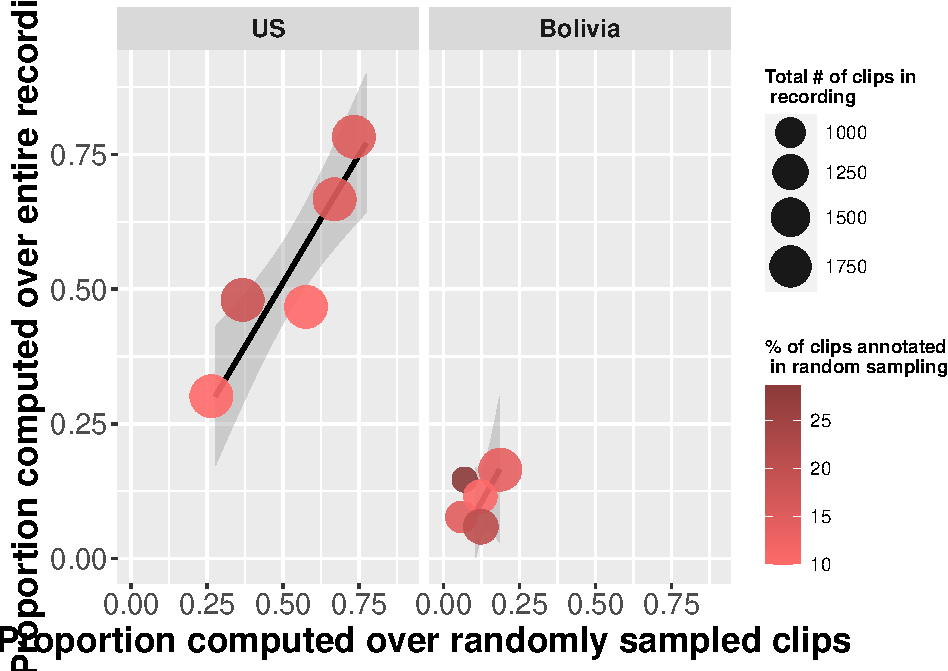
\includegraphics{validation_results_files/figure-latex/cds plot-1.pdf}

\begin{Shaded}
\begin{Highlighting}[]
\KeywordTok{jpeg}\NormalTok{(}\StringTok{"/Users/megcychosz/Google Drive/biling_CDS/results/figures/cds_plot.jpeg"}\NormalTok{, }\DataTypeTok{height =} \DecValTok{500}\NormalTok{, }\DataTypeTok{width =} \DecValTok{500}\NormalTok{)}
\NormalTok{cds_plot}
\KeywordTok{dev.off}\NormalTok{()}
\end{Highlighting}
\end{Shaded}

\begin{verbatim}
## pdf 
##   2
\end{verbatim}

\hypertarget{part-iii-language-across-random-and-questionnaire-methods}{%
\subsubsection{Part III: language across random and questionnaire methods}\label{part-iii-language-across-random-and-questionnaire-methods}}

\begin{Shaded}
\begin{Highlighting}[]
\CommentTok{# enter questionnaire estimates}
\NormalTok{ques <-}\StringTok{ }\KeywordTok{data.frame}\NormalTok{(}\StringTok{"id"}\NormalTok{=}\KeywordTok{c}\NormalTok{(}\StringTok{"179"}\NormalTok{, }\StringTok{"198-9mo"}\NormalTok{, }\StringTok{"199"}\NormalTok{, }\StringTok{"261-8mo"}\NormalTok{, }\StringTok{"267-12mo"}\NormalTok{), }
                   \StringTok{"ques_est"}\NormalTok{=}\KeywordTok{c}\NormalTok{(}\StringTok{".71"}\NormalTok{, }\StringTok{".57"}\NormalTok{, }\StringTok{".94"}\NormalTok{, }\StringTok{".69"}\NormalTok{, }\StringTok{".87"}\NormalTok{))}

\NormalTok{ques_tbl <-}\StringTok{ }\NormalTok{plot_data }\OperatorTok
\StringTok{  }\KeywordTok{filter}\NormalTok{(location}\OperatorTok{==}\StringTok{'US'}\NormalTok{) }\OperatorTok
\StringTok{  }\KeywordTok{merge}\NormalTok{(., ques, }\DataTypeTok{by=}\StringTok{'id'}\NormalTok{) }\OperatorTok
\StringTok{  }\KeywordTok{distinct_at}\NormalTok{(., }\KeywordTok{vars}\NormalTok{(method, id), }\DataTypeTok{.keep_all =}\NormalTok{ T) }\OperatorTok
\StringTok{  }\KeywordTok{select}\NormalTok{(}\OperatorTok{-}\NormalTok{percen_ofallclips_drawn, }\OperatorTok{-}\NormalTok{percen_mxd, }\OperatorTok{-}\NormalTok{percen_que, }\OperatorTok{-}\NormalTok{speech_clips, }\OperatorTok{-}\NormalTok{total, }\OperatorTok{-}\NormalTok{gender, }\OperatorTok{-}\NormalTok{location, }\OperatorTok{-}\NormalTok{num_clips) }\OperatorTok
\StringTok{  }\KeywordTok{mutate}\NormalTok{(}\DataTypeTok{percen_span =} \KeywordTok{round}\NormalTok{(percen_span,}\DecValTok{2}\NormalTok{)) }\OperatorTok
\StringTok{  }\KeywordTok{spread}\NormalTok{(}\StringTok{"method"}\NormalTok{, }\StringTok{"percen_span"}\NormalTok{) }\OperatorTok
\StringTok{  }\KeywordTok{relocate}\NormalTok{(id, random, complete, ques_est)}

\CommentTok{# compute correlations}
\NormalTok{ques_random_cors <-}\StringTok{ }\NormalTok{ques_tbl }\OperatorTok
\StringTok{  }\KeywordTok{mutate}\NormalTok{(}\DataTypeTok{ques_est =} \KeywordTok{as.numeric}\NormalTok{(ques_est)) }\OperatorTok
\StringTok{  }\KeywordTok{summarize}\NormalTok{(., }\KeywordTok{paste}\NormalTok{(}\StringTok{"r="}\NormalTok{,}\KeywordTok{round}\NormalTok{(}\KeywordTok{cor.test}\NormalTok{(ques_est, random)}\OperatorTok{$}\NormalTok{estimate,}\DecValTok{2}\NormalTok{),}\StringTok{","}\NormalTok{,}\StringTok{"p="}\NormalTok{,}\KeywordTok{round}\NormalTok{(}\KeywordTok{cor.test}\NormalTok{(ques_est, random)}\OperatorTok{$}\NormalTok{p.value,}\DecValTok{2}\NormalTok{)))}
\NormalTok{ques_complete_cors <-}\StringTok{ }\NormalTok{ques_tbl }\OperatorTok
\StringTok{  }\KeywordTok{mutate}\NormalTok{(}\DataTypeTok{ques_est =} \KeywordTok{as.numeric}\NormalTok{(ques_est)) }\OperatorTok
\StringTok{  }\KeywordTok{summarize}\NormalTok{(., }\KeywordTok{paste}\NormalTok{(}\StringTok{"r="}\NormalTok{,}\KeywordTok{round}\NormalTok{(}\KeywordTok{cor.test}\NormalTok{(ques_est, complete)}\OperatorTok{$}\NormalTok{estimate,}\DecValTok{2}\NormalTok{),}\StringTok{","}\NormalTok{,}\StringTok{"p="}\NormalTok{,}\KeywordTok{round}\NormalTok{(}\KeywordTok{cor.test}\NormalTok{(ques_est, complete)}\OperatorTok{$}\NormalTok{p.value,}\DecValTok{2}\NormalTok{)))}

\CommentTok{# create table}
\NormalTok{knitr}\OperatorTok{::}\KeywordTok{kable}\NormalTok{(ques_tbl, }\DataTypeTok{caption =} \StringTok{'Spanish language estimates in U.S. corpus, by child and estimation method.'}\NormalTok{, }
             \DataTypeTok{booktabs=}\NormalTok{T, }
             \DataTypeTok{row.names =} \OtherTok{FALSE}\NormalTok{, }
             \DataTypeTok{col.names =} \KeywordTok{c}\NormalTok{(}\StringTok{"Child ID"}\NormalTok{, }\StringTok{"Random"}\NormalTok{, }\StringTok{"All-day"}\NormalTok{, }\StringTok{"Parental Questionnaire"}\NormalTok{)) }\OperatorTok\StringTok{ }
\StringTok{  }\KeywordTok{kable_styling}\NormalTok{() }\OperatorTok
\StringTok{  }\KeywordTok{add_header_above}\NormalTok{(}\KeywordTok{c}\NormalTok{(}\StringTok{" "}\NormalTok{ =}\StringTok{ }\DecValTok{1}\NormalTok{, }\StringTok{"From daylong recording"}\NormalTok{ =}\StringTok{ }\DecValTok{2}\NormalTok{, }\StringTok{" "}\NormalTok{ =}\StringTok{ }\DecValTok{1}\NormalTok{)) }\OperatorTok
\StringTok{  }\NormalTok{kableExtra}\OperatorTok{::}\KeywordTok{kable_styling}\NormalTok{(}\DataTypeTok{latex_options =} \StringTok{"hold_position"}\NormalTok{)}
\end{Highlighting}
\end{Shaded}

\begin{table}[!h]

\caption{(\#tab:make table for questionnaire method)Spanish language estimates in U.S. corpus, by child and estimation method.}
\centering
\begin{tabular}[t]{lrrl}
\toprule
\multicolumn{1}{c}{ } & \multicolumn{2}{c}{From daylong recording} & \multicolumn{1}{c}{ } \\
\cmidrule(l{3pt}r{3pt}){2-3}
Child ID & Random & All-day & Parental Questionnaire\\
\midrule
179 & 0.57 & 0.57 & .71\\
198-9mo & 0.87 & 0.78 & .57\\
199 & 0.76 & 0.70 & .94\\
261-8mo & 0.69 & 0.65 & .69\\
267-12mo & 0.92 & 0.92 & .87\\
\bottomrule
\end{tabular}
\end{table}

\begin{Shaded}
\begin{Highlighting}[]
\CommentTok{# we also want to know what the results are for the combination of CDS*Spanish, not just Spanish}
\NormalTok{reg_annon <-}\StringTok{ }\NormalTok{data_annon }\OperatorTok
\StringTok{  }\KeywordTok{filter}\NormalTok{(addressee}\OperatorTok{==}\StringTok{'Adult2TargetChild'} \OperatorTok{|}\StringTok{ }\NormalTok{addressee}\OperatorTok{==}\StringTok{'Otherchild2TargetChild'}\NormalTok{) }\OperatorTok\StringTok{ }\CommentTok{# only CDS clips}
\StringTok{  }\KeywordTok{group_by}\NormalTok{(id, method) }\OperatorTok
\StringTok{  }\KeywordTok{distinct_at}\NormalTok{(., }\KeywordTok{vars}\NormalTok{(file_name, addressee), }\DataTypeTok{.keep_all =}\NormalTok{ T) }\OperatorTok\StringTok{ }\CommentTok{# don't record multiple speakers speaking the same register}
\StringTok{  }\KeywordTok{mutate}\NormalTok{(}\DataTypeTok{total_cds_annotations =} \KeywordTok{NROW}\NormalTok{(file_name))}\CommentTok{#}

\NormalTok{span_cds_tbl <-}\StringTok{ }\NormalTok{reg_annon }\OperatorTok\StringTok{ }
\StringTok{  }\KeywordTok{group_by}\NormalTok{(id, method) }\OperatorTok
\StringTok{  }\KeywordTok{filter}\NormalTok{(addressee}\OperatorTok{==}\StringTok{'Adult2TargetChild'} \OperatorTok{|}\StringTok{ }\NormalTok{addressee}\OperatorTok{==}\StringTok{'Otherchild2TargetChild'} \OperatorTok{&}\StringTok{ }\NormalTok{location}\OperatorTok{==}\StringTok{'US'}\NormalTok{) }\OperatorTok\StringTok{ }\CommentTok{# only CDS clips}
\StringTok{  }\KeywordTok{merge}\NormalTok{(., ques, }\DataTypeTok{by=}\StringTok{'id'}\NormalTok{) }\OperatorTok
\StringTok{  }\KeywordTok{filter}\NormalTok{(language}\OperatorTok{==}\StringTok{'Spanish'}\NormalTok{) }\OperatorTok\StringTok{ }\CommentTok{# only Spanish clips}
\StringTok{  }\KeywordTok{group_by}\NormalTok{(method) }\OperatorTok
\StringTok{  }\KeywordTok{distinct}\NormalTok{(file_name, }\DataTypeTok{.keep_all =}\NormalTok{ T) }\OperatorTok\StringTok{ }
\StringTok{  }\KeywordTok{group_by}\NormalTok{(id, method) }\OperatorTok
\StringTok{  }\KeywordTok{mutate}\NormalTok{(}\DataTypeTok{n_span_cds =} \KeywordTok{n}\NormalTok{()) }\OperatorTok\StringTok{ }\CommentTok{# # of CDS clips where Spanish was spoken}
\StringTok{  }\KeywordTok{distinct_at}\NormalTok{(., }\KeywordTok{vars}\NormalTok{(id, method), }\DataTypeTok{.keep_all =}\NormalTok{ T) }\OperatorTok
\StringTok{  }\KeywordTok{mutate}\NormalTok{(}\DataTypeTok{percen_span_cds =} \KeywordTok{round}\NormalTok{(n_span_cds }\OperatorTok{/}\StringTok{ }\NormalTok{total_cds_annotations,}\DecValTok{2}\NormalTok{)) }\OperatorTok
\StringTok{  }\KeywordTok{select}\NormalTok{(method, percen_span_cds, id, ques_est) }\OperatorTok
\StringTok{  }\KeywordTok{spread}\NormalTok{(}\StringTok{"method"}\NormalTok{, }\StringTok{"percen_span_cds"}\NormalTok{) }\OperatorTok
\StringTok{  }\KeywordTok{relocate}\NormalTok{(id, random, complete, ques_est) }

\CommentTok{# compute correlations}
\KeywordTok{cor.test}\NormalTok{(}\KeywordTok{as.numeric}\NormalTok{(span_cds_tbl}\OperatorTok{$}\NormalTok{ques_est), span_cds_tbl}\OperatorTok{$}\NormalTok{complete)}
\end{Highlighting}
\end{Shaded}

\begin{verbatim}
## 
##  Pearson's product-moment correlation
## 
## data:  as.numeric(span_cds_tbl$ques_est) and span_cds_tbl$complete
## t = 1.022, df = 3, p-value = 0.382
## alternative hypothesis: true correlation is not equal to 0
## 95 percent confidence interval:
##  -0.6781348  0.9600192
## sample estimates:
##       cor 
## 0.5081637
\end{verbatim}

\begin{Shaded}
\begin{Highlighting}[]
\KeywordTok{cor.test}\NormalTok{(}\KeywordTok{as.numeric}\NormalTok{(span_cds_tbl}\OperatorTok{$}\NormalTok{ques_est), span_cds_tbl}\OperatorTok{$}\NormalTok{random)}
\end{Highlighting}
\end{Shaded}

\begin{verbatim}
## 
##  Pearson's product-moment correlation
## 
## data:  as.numeric(span_cds_tbl$ques_est) and span_cds_tbl$random
## t = 0.12188, df = 3, p-value = 0.9107
## alternative hypothesis: true correlation is not equal to 0
## 95 percent confidence interval:
##  -0.8656838  0.8969149
## sample estimates:
##       cor 
## 0.0701952
\end{verbatim}

\begin{Shaded}
\begin{Highlighting}[]
\CommentTok{# create table}
\NormalTok{knitr}\OperatorTok{::}\KeywordTok{kable}\NormalTok{(span_cds_tbl, }\DataTypeTok{caption =} \StringTok{'Spanish language in child-directed speech }\CharTok{\textbackslash{}n}\StringTok{ estimates in U.S. corpus, by child and estimation method.'}\NormalTok{, }
             \DataTypeTok{booktabs=}\NormalTok{T, }
             \DataTypeTok{row.names =} \OtherTok{FALSE}\NormalTok{, }
             \DataTypeTok{col.names =} \KeywordTok{c}\NormalTok{(}\StringTok{"Child ID"}\NormalTok{, }\StringTok{"Random"}\NormalTok{, }\StringTok{"All-day"}\NormalTok{, }\StringTok{"Parental Questionnaire"}\NormalTok{)) }\OperatorTok\StringTok{ }
\StringTok{  }\KeywordTok{kable_styling}\NormalTok{() }\OperatorTok
\StringTok{  }\KeywordTok{add_header_above}\NormalTok{(}\KeywordTok{c}\NormalTok{(}\StringTok{" "}\NormalTok{ =}\StringTok{ }\DecValTok{1}\NormalTok{, }\StringTok{"From daylong recording"}\NormalTok{ =}\StringTok{ }\DecValTok{2}\NormalTok{, }\StringTok{" "}\NormalTok{ =}\StringTok{ }\DecValTok{1}\NormalTok{)) }\OperatorTok
\StringTok{  }\NormalTok{kableExtra}\OperatorTok{::}\KeywordTok{kable_styling}\NormalTok{(}\DataTypeTok{latex_options =} \StringTok{"hold_position"}\NormalTok{)}
\end{Highlighting}
\end{Shaded}

\begin{table}[!h]

\caption{(\#tab:make table for questionnaire method)Spanish language in child-directed speech 
 estimates in U.S. corpus, by child and estimation method.}
\centering
\begin{tabular}[t]{lrrl}
\toprule
\multicolumn{1}{c}{ } & \multicolumn{2}{c}{From daylong recording} & \multicolumn{1}{c}{ } \\
\cmidrule(l{3pt}r{3pt}){2-3}
Child ID & Random & All-day & Parental Questionnaire\\
\midrule
179 & 0.53 & 0.52 & .71\\
198-9mo & 0.78 & 0.64 & .57\\
199 & 0.64 & 0.66 & .94\\
261-8mo & 0.55 & 0.48 & .69\\
267-12mo & 0.82 & 0.87 & .87\\
\bottomrule
\end{tabular}
\end{table}

\begin{Shaded}
\begin{Highlighting}[]
\CommentTok{# for later}
\NormalTok{per_ann <-}\StringTok{ }\NormalTok{plot_data }\OperatorTok
\StringTok{  }\KeywordTok{filter}\NormalTok{(method}\OperatorTok{==}\StringTok{'random'} \OperatorTok{&}\StringTok{ }\NormalTok{location}\OperatorTok{==}\StringTok{'US'}\NormalTok{) }\OperatorTok
\StringTok{  }\KeywordTok{select}\NormalTok{(id, percen_ofallclips_drawn)}

\NormalTok{ques_plot <-}\StringTok{ }\NormalTok{plot_data }\OperatorTok
\StringTok{  }\KeywordTok{filter}\NormalTok{(location}\OperatorTok{==}\StringTok{'US'}\NormalTok{) }\OperatorTok
\StringTok{  }\KeywordTok{merge}\NormalTok{(., ques, }\DataTypeTok{by=}\StringTok{'id'}\NormalTok{) }\OperatorTok
\StringTok{  }\KeywordTok{distinct_at}\NormalTok{(., }\KeywordTok{vars}\NormalTok{(method, id), }\DataTypeTok{.keep_all =}\NormalTok{ T) }\OperatorTok
\StringTok{  }\KeywordTok{select}\NormalTok{(}\OperatorTok{-}\NormalTok{percen_que, }\OperatorTok{-}\NormalTok{percen_ofallclips_drawn, }\OperatorTok{-}\NormalTok{percen_mxd, }\OperatorTok{-}\NormalTok{speech_clips, }\OperatorTok{-}\NormalTok{total) }\OperatorTok
\StringTok{  }\KeywordTok{spread}\NormalTok{(}\StringTok{"method"}\NormalTok{, }\StringTok{"percen_span"}\NormalTok{) }\OperatorTok
\StringTok{  }\KeywordTok{select}\NormalTok{(}\OperatorTok{-}\NormalTok{complete) }\OperatorTok
\StringTok{  }\KeywordTok{merge}\NormalTok{(., per_ann, }\DataTypeTok{by=}\StringTok{'id'}\NormalTok{) }\OperatorTok
\StringTok{  }\KeywordTok{distinct}\NormalTok{(id, }\DataTypeTok{.keep_all =}\NormalTok{ T) }\OperatorTok
\KeywordTok{ggplot}\NormalTok{(., }\KeywordTok{aes}\NormalTok{(}\KeywordTok{as.numeric}\NormalTok{(ques_est), random)) }\OperatorTok{+}
\StringTok{  }\KeywordTok{geom_smooth}\NormalTok{(}\DataTypeTok{method =} \StringTok{"lm"}\NormalTok{, }\DataTypeTok{color=}\StringTok{"black"}\NormalTok{, }\DataTypeTok{se=}\OtherTok{FALSE}\NormalTok{) }\OperatorTok{+}
\StringTok{  }\KeywordTok{geom_jitter}\NormalTok{(}\KeywordTok{aes}\NormalTok{(}\DataTypeTok{size=}\NormalTok{num_clips,}\DataTypeTok{color=}\KeywordTok{round}\NormalTok{(percen_ofallclips_drawn,}\DecValTok{2}\NormalTok{)),}\DataTypeTok{alpha=}\NormalTok{.}\DecValTok{9}\NormalTok{,}\DataTypeTok{position =} \KeywordTok{position_jitter}\NormalTok{(}\DataTypeTok{width =} \FloatTok{0.07}\NormalTok{, }\DataTypeTok{height =} \FloatTok{.01}\NormalTok{)) }\OperatorTok{+}
\StringTok{  }\KeywordTok{scale_size_continuous}\NormalTok{(}\DataTypeTok{range =} \KeywordTok{c}\NormalTok{(}\DecValTok{5}\NormalTok{, }\DecValTok{9}\NormalTok{)) }\OperatorTok{+}\StringTok{ }
\StringTok{  }\KeywordTok{scale_colour_gradient}\NormalTok{(}\DataTypeTok{low=}\StringTok{'indianred1'}\NormalTok{, }\DataTypeTok{high =} \StringTok{'indianred4'}\NormalTok{) }\OperatorTok{+}
\StringTok{  }\KeywordTok{ylab}\NormalTok{(}\StringTok{"Proportion computed from }\CharTok{\textbackslash{}n}\StringTok{ background questionnaire"}\NormalTok{) }\OperatorTok{+}\StringTok{ }
\StringTok{  }\KeywordTok{xlab}\NormalTok{(}\StringTok{"Proportion computed over }\CharTok{\textbackslash{}n}\StringTok{ randomly sampled clips"}\NormalTok{) }\OperatorTok{+}\StringTok{ }
\StringTok{  }\KeywordTok{ylim}\NormalTok{(}\DecValTok{0}\NormalTok{,}\DecValTok{1}\NormalTok{) }\OperatorTok{+}
\StringTok{  }\KeywordTok{xlim}\NormalTok{(}\DecValTok{0}\NormalTok{,}\DecValTok{1}\NormalTok{)}\OperatorTok{+}
\StringTok{  }\KeywordTok{labs}\NormalTok{(}\DataTypeTok{col=}\StringTok{'% of clips drawn }\CharTok{\textbackslash{}n}\StringTok{ in random sampling'}\NormalTok{) }\OperatorTok{+}\StringTok{ }
\StringTok{       }\CommentTok{#title = 'Proportion of Spanish clips \textbackslash{}n in U.S. corpus: random sampling and background questionnaire methods') +}
\StringTok{ }\KeywordTok{theme}\NormalTok{(}\DataTypeTok{title =} \KeywordTok{element_text}\NormalTok{(}\DataTypeTok{size=}\DecValTok{18}\NormalTok{, }\DataTypeTok{face=}\StringTok{"bold"}\NormalTok{),}
   \DataTypeTok{axis.text=}\KeywordTok{element_text}\NormalTok{(}\DataTypeTok{size=}\DecValTok{14}\NormalTok{),}
      \DataTypeTok{axis.title=}\KeywordTok{element_text}\NormalTok{(}\DataTypeTok{size=}\DecValTok{17}\NormalTok{,}\DataTypeTok{face=}\StringTok{"bold"}\NormalTok{),}
      \DataTypeTok{legend.title =} \KeywordTok{element_text}\NormalTok{(}\DataTypeTok{size=}\DecValTok{15}\NormalTok{)) }\OperatorTok{+}
\StringTok{      }\KeywordTok{guides}\NormalTok{(}\DataTypeTok{size=}\KeywordTok{guide_legend}\NormalTok{(}\DataTypeTok{title=}\StringTok{"Total # of clips in }\CharTok{\textbackslash{}n}\StringTok{ recording"}\NormalTok{))}
\NormalTok{ques_plot}
\end{Highlighting}
\end{Shaded}

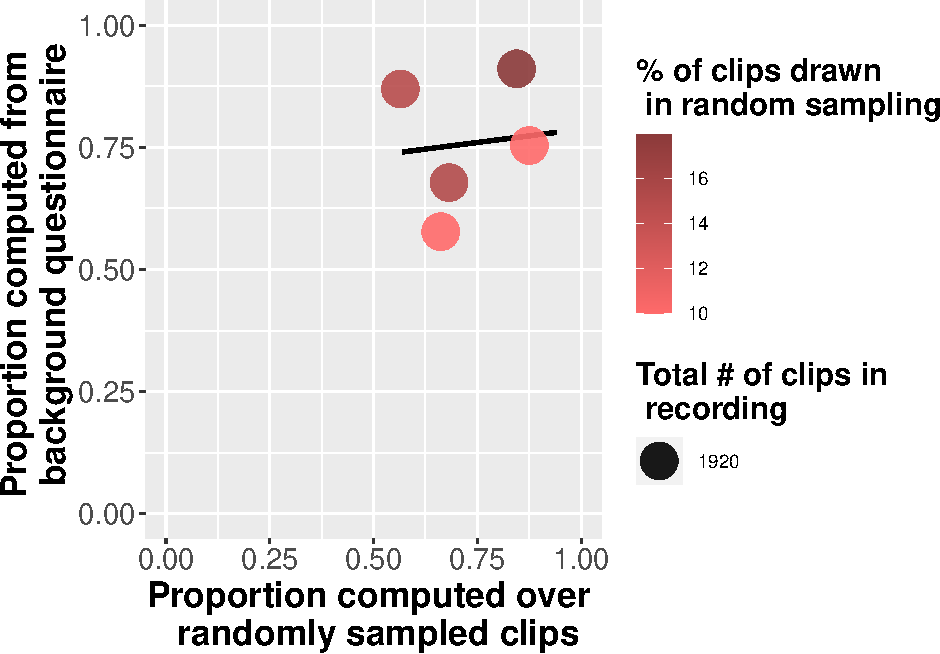
\includegraphics{validation_results_files/figure-latex/questionnaire plot-1.pdf}

\begin{Shaded}
\begin{Highlighting}[]
\KeywordTok{jpeg}\NormalTok{(}\StringTok{"/Users/megcychosz/Google Drive/biling_CDS/results/figures/ques_plot.jpeg"}\NormalTok{, }\DataTypeTok{height =} \DecValTok{500}\NormalTok{, }\DataTypeTok{width =} \DecValTok{600}\NormalTok{)}
\NormalTok{ques_plot}
\KeywordTok{dev.off}\NormalTok{()}
\end{Highlighting}
\end{Shaded}

\begin{verbatim}
## pdf 
##   2
\end{verbatim}

\hypertarget{part-i-running-variance}{%
\subsubsection{Part I: Running variance}\label{part-i-running-variance}}

\begin{Shaded}
\begin{Highlighting}[]
\NormalTok{random}\OperatorTok{$}\NormalTok{id <-}\StringTok{ }\NormalTok{plyr}\OperatorTok{::}\KeywordTok{mapvalues}\NormalTok{(random}\OperatorTok{$}\NormalTok{id, }
                \DataTypeTok{from=}\KeywordTok{c}\NormalTok{(}\StringTok{"198-9mo"}\NormalTok{, }\StringTok{"261-8mo"}\NormalTok{, }\StringTok{"267-12mo"}\NormalTok{), }
                \DataTypeTok{to=}\KeywordTok{c}\NormalTok{(}\StringTok{"198"}\NormalTok{, }\StringTok{"261"}\NormalTok{, }\StringTok{"267"}\NormalTok{))}

\CommentTok{# only doing for CDS first - filter for other languages for language}
\NormalTok{cds_var <-}\StringTok{ }\NormalTok{random }\OperatorTok\StringTok{ }
\StringTok{  }\KeywordTok{group_by}\NormalTok{(id) }\OperatorTok
\StringTok{  }\KeywordTok{mutate}\NormalTok{(}\DataTypeTok{total=}\KeywordTok{n}\NormalTok{()) }\OperatorTok\StringTok{ }\CommentTok{# total clips drawn & listened to}
\StringTok{  }\KeywordTok{filter}\NormalTok{(researcher_present}\OperatorTok{!=}\StringTok{'1'} \OperatorTok{&}\StringTok{ }\NormalTok{sleeping}\OperatorTok{!=}\StringTok{'1'} \OperatorTok{&}\StringTok{ }\NormalTok{percents_voc}\OperatorTok{>}\DecValTok{0}\NormalTok{) }\OperatorTok\StringTok{ }\CommentTok{# criteria for draw, but don't listen}
\StringTok{  }\KeywordTok{distinct}\NormalTok{(file_name, }\DataTypeTok{.keep_all =}\NormalTok{ T) }\OperatorTok
\StringTok{  }\KeywordTok{mutate}\NormalTok{(}\DataTypeTok{annotation_num =} \KeywordTok{as.numeric}\NormalTok{(}\DecValTok{1}\OperatorTok{:}\KeywordTok{n}\NormalTok{())) }\OperatorTok\StringTok{ }\CommentTok{# total clips annotated for lang/reg/childvoc/media, not just drawn}
\StringTok{  }\KeywordTok{select}\NormalTok{(}\OperatorTok{-}\NormalTok{Otherchild2OtherChild, }\OperatorTok{-}\NormalTok{Otherchild2adults, }\OperatorTok{-}\NormalTok{Otherchild2unsure, }\OperatorTok{-}\NormalTok{Adult2OtherChild, }\OperatorTok{-}\NormalTok{Adult2Others, }\OperatorTok{-}\NormalTok{Adult2unsure) }\OperatorTok
\StringTok{  }\KeywordTok{gather}\NormalTok{(}\StringTok{"addressee"}\NormalTok{, }\StringTok{"language"}\NormalTok{, Adult2TargetChild, Otherchild2TargetChild) }\OperatorTok
\StringTok{  }\KeywordTok{distinct_at}\NormalTok{(., }\KeywordTok{vars}\NormalTok{(file_name, timestamp_HHMMSS), }\DataTypeTok{.keep_all =}\NormalTok{ T) }\OperatorTok\StringTok{ }\CommentTok{# CDS only gets counted 1x/clip; maintains clips drawn twice}
\StringTok{  }\KeywordTok{select}\NormalTok{(}\OperatorTok{-}\NormalTok{addressee)}


\NormalTok{cds_var}\OperatorTok{$}\NormalTok{cds_cts <-}\StringTok{ }\NormalTok{plyr}\OperatorTok{::}\KeywordTok{mapvalues}\NormalTok{(cds_var}\OperatorTok{$}\NormalTok{language, }
                \DataTypeTok{from=}\KeywordTok{c}\NormalTok{(}\StringTok{"Categorize language to target child"}\NormalTok{, }\StringTok{"English/Quechua"}\NormalTok{, }\StringTok{"Mixed"}\NormalTok{, }\StringTok{"Spanish"}\NormalTok{, }\StringTok{"Unsure"}\NormalTok{), }
                \DataTypeTok{to=}\KeywordTok{c}\NormalTok{(}\StringTok{"0"}\NormalTok{, }\StringTok{"1"}\NormalTok{, }\StringTok{"1"}\NormalTok{, }\StringTok{"1"}\NormalTok{, }\StringTok{"1"}\NormalTok{)) }\CommentTok{# where 'cat lang...' are ADS or OCDS}
\NormalTok{cds_var}\OperatorTok{$}\NormalTok{cds_cts <-}\StringTok{ }\KeywordTok{as.numeric}\NormalTok{(cds_var}\OperatorTok{$}\NormalTok{cds_cts)}
\NormalTok{cds_var}\OperatorTok{$}\NormalTok{total <-}\StringTok{ }\KeywordTok{as.numeric}\NormalTok{(cds_var}\OperatorTok{$}\NormalTok{total)}

\NormalTok{cds_rolling <-}\StringTok{ }\NormalTok{cds_var }\OperatorTok
\StringTok{  }\KeywordTok{group_by}\NormalTok{(id) }\OperatorTok
\StringTok{  }\KeywordTok{mutate}\NormalTok{(}\DataTypeTok{cds_running_cts =} \KeywordTok{as.numeric}\NormalTok{(}\KeywordTok{cumsum}\NormalTok{(cds_cts))) }\OperatorTok
\StringTok{  }\KeywordTok{mutate}\NormalTok{(}\DataTypeTok{roll_prop_cds =}\NormalTok{ cds_running_cts }\OperatorTok{/}\StringTok{ }\NormalTok{annotation_num,}
         \DataTypeTok{roll_mean_cds =} \KeywordTok{rollmean}\NormalTok{(roll_prop_cds, }\DataTypeTok{k=}\DecValTok{10}\NormalTok{, }\DataTypeTok{fill =} \OtherTok{NA}\NormalTok{),}
         \DataTypeTok{roll_sd_cds =} \KeywordTok{rollapply}\NormalTok{(roll_prop_cds, }\DataTypeTok{width=}\DecValTok{10}\NormalTok{, }\DataTypeTok{FUN=}\NormalTok{sd, }\DataTypeTok{fill=}\OtherTok{NA}\NormalTok{))}

\CommentTok{# running binomial confidence interval (wilson)}
\NormalTok{cds_rolling2 <-}\StringTok{ }\NormalTok{cds_rolling }\OperatorTok
\StringTok{  }\KeywordTok{group_by}\NormalTok{(id, annotation_num) }\OperatorTok\StringTok{ }\CommentTok{# group by id and sample size}
\StringTok{  }\KeywordTok{summarize}\NormalTok{(}\DataTypeTok{cis =} \KeywordTok{binom.confint}\NormalTok{(cds_running_cts, annotation_num, }\DataTypeTok{methods =} \StringTok{'wilson'}\NormalTok{, }\DataTypeTok{conf.level =} \FloatTok{.95}\NormalTok{)) }\OperatorTok
\StringTok{  }\KeywordTok{merge}\NormalTok{(., cds_rolling, }\DataTypeTok{by =} \KeywordTok{c}\NormalTok{(}\StringTok{'id'}\NormalTok{, }\StringTok{'annotation_num'}\NormalTok{)) }

\CommentTok{# for models, compute binomial confidence interval in 5-clip batches}
\CommentTok{#cds_batches <- cds_rolling %>%}
\CommentTok{#  group_by(id) %>%}
\CommentTok{#  mutate(five_clip_batch = as.integer(gl(n(), 5, n())) * 5,}
\CommentTok{#         five_clip_batch = replace(five_clip_batch,  ave(five_clip_batch, five_clip_batch, FUN = length) < 5, NA)) %>% }
\CommentTok{#  ungroup %>% }
\CommentTok{#  fill(five_clip_batch) #%>%}

\CommentTok{#cds_batches2 <- cds_batches %>%}
\CommentTok{#  group_by(id, five_clip_batch) %>%}
\CommentTok{#  summarize(five_cis = binom.confint(cds_running_cts, 5, methods = 'wilson', conf.level = .95)) %>%}
\CommentTok{#  merge(., cds_batches, by = c('id', 'five_clip_batch'))}
\end{Highlighting}
\end{Shaded}

\begin{Shaded}
\begin{Highlighting}[]
\NormalTok{cds_var_plot <-}\StringTok{ }\NormalTok{cds_rolling2 }\OperatorTok
\CommentTok{#filter(roll_sd_cds!='NA') %>% # remove rows where variance wasn't estimated}
\KeywordTok{mutate}\NormalTok{(}\DataTypeTok{mean_ci =}\NormalTok{ cis}\OperatorTok{$}\NormalTok{mean,}
       \DataTypeTok{upper_ci =}\NormalTok{ cis}\OperatorTok{$}\NormalTok{upper,}
       \DataTypeTok{lower_ci =}\NormalTok{ cis}\OperatorTok{$}\NormalTok{lower) }\OperatorTok\StringTok{  }
\KeywordTok{ggplot}\NormalTok{(., }\KeywordTok{aes}\NormalTok{(annotation_num, roll_prop_cds)) }\OperatorTok{+}
\StringTok{  }\CommentTok{#geom_line(aes(y=rollapply(roll_prop_cds, 10, FUN=sd, fill=NA))) +}
\StringTok{  }\KeywordTok{geom_ribbon}\NormalTok{(}\KeywordTok{aes}\NormalTok{(}\DataTypeTok{ymax=}\NormalTok{upper_ci, }\DataTypeTok{ymin=}\NormalTok{lower_ci), }\DataTypeTok{fill=}\StringTok{'lightblue'}\NormalTok{, }\DataTypeTok{color=}\StringTok{'deepskyblue4'}\NormalTok{) }\OperatorTok{+}\StringTok{  }
\StringTok{    }\KeywordTok{geom_line}\NormalTok{(}\KeywordTok{aes}\NormalTok{(}\DataTypeTok{y=}\NormalTok{mean_ci), }\DataTypeTok{color=}\StringTok{'gray40'}\NormalTok{, }\DataTypeTok{size=}\NormalTok{.}\DecValTok{8}\NormalTok{) }\OperatorTok{+}\StringTok{ }
\StringTok{  }\KeywordTok{xlab}\NormalTok{(}\StringTok{"# of clips annotated"}\NormalTok{) }\OperatorTok{+}\StringTok{ }
\StringTok{  }\KeywordTok{ylab}\NormalTok{(}\StringTok{"CDS estimation and variance"}\NormalTok{) }\OperatorTok{+}\StringTok{ }
\StringTok{  }\KeywordTok{facet_wrap}\NormalTok{(}\OperatorTok{~}\NormalTok{id, }\DataTypeTok{scales =} \StringTok{"free"}\NormalTok{) }\OperatorTok{+}
\StringTok{  }\CommentTok{#title = 'Variance in child-directed estimation as a function of clips annotated') +}
\StringTok{ }\KeywordTok{theme}\NormalTok{(}\DataTypeTok{title =} \KeywordTok{element_text}\NormalTok{(}\DataTypeTok{size=}\DecValTok{12}\NormalTok{),}
   \DataTypeTok{axis.text=}\KeywordTok{element_text}\NormalTok{(}\DataTypeTok{size=}\DecValTok{8}\NormalTok{),}
      \DataTypeTok{axis.title=}\KeywordTok{element_text}\NormalTok{(}\DataTypeTok{size=}\DecValTok{17}\NormalTok{,}\DataTypeTok{face=}\StringTok{"bold"}\NormalTok{),}
      \DataTypeTok{legend.title =} \KeywordTok{element_text}\NormalTok{(}\DataTypeTok{size=}\DecValTok{15}\NormalTok{)) }\OperatorTok{+}
\StringTok{  }\KeywordTok{labs}\NormalTok{(}\DataTypeTok{caption =} \StringTok{"Number of clips annotated refers to those annotated for language, speech register, child vocalizations, and/or media."}\NormalTok{)}
\NormalTok{cds_var_plot}
\end{Highlighting}
\end{Shaded}

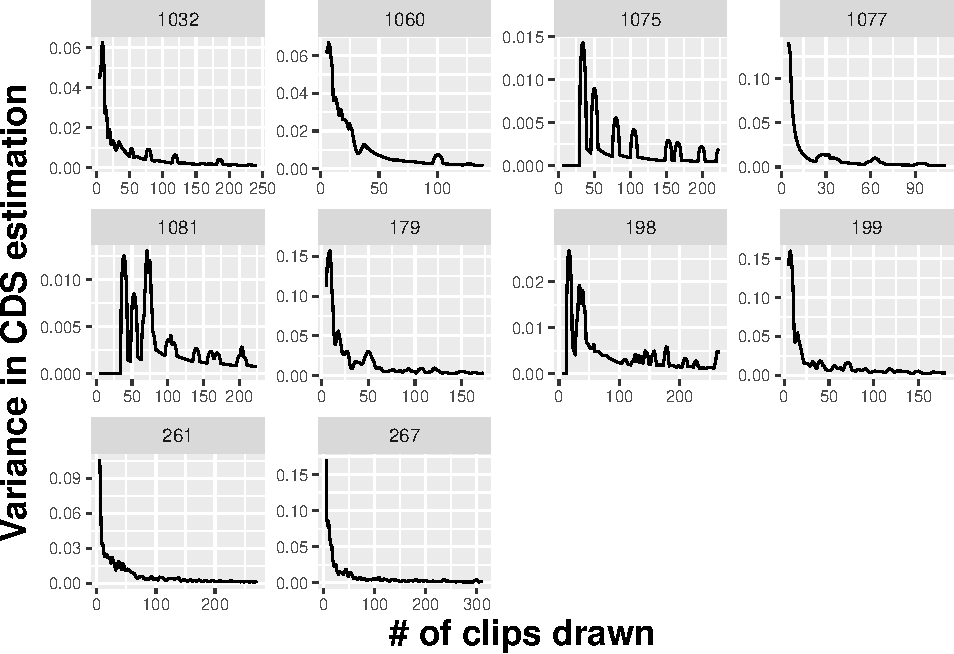
\includegraphics{validation_results_files/figure-latex/plot rolling CDS variances-1.pdf}

\begin{Shaded}
\begin{Highlighting}[]
\KeywordTok{jpeg}\NormalTok{(}\StringTok{"/Users/megcychosz/Google Drive/biling_CDS/results/figures/cds_CI_var_plot.jpeg"}\NormalTok{, }\DataTypeTok{height =} \DecValTok{450}\NormalTok{, }\DataTypeTok{width =} \DecValTok{700}\NormalTok{)}
\NormalTok{cds_var_plot}
\KeywordTok{dev.off}\NormalTok{()}
\end{Highlighting}
\end{Shaded}

\begin{verbatim}
## pdf 
##   2
\end{verbatim}

\begin{Shaded}
\begin{Highlighting}[]
\CommentTok{# now calculate rolling variances for US (Spanish)}
\NormalTok{span_var <-}\StringTok{ }\NormalTok{random }\OperatorTok\StringTok{ }
\StringTok{  }\KeywordTok{group_by}\NormalTok{(id) }\OperatorTok
\StringTok{  }\KeywordTok{mutate}\NormalTok{(}\DataTypeTok{total=}\KeywordTok{n}\NormalTok{()) }\OperatorTok\StringTok{ }\CommentTok{# total clips drawn }
\StringTok{  }\KeywordTok{filter}\NormalTok{(researcher_present}\OperatorTok{!=}\StringTok{'1'} \OperatorTok{&}\StringTok{ }\NormalTok{sleeping}\OperatorTok{!=}\StringTok{'1'} \OperatorTok{&}\StringTok{ }\NormalTok{percents_voc}\OperatorTok{>}\DecValTok{0}\NormalTok{) }\OperatorTok\StringTok{ }\CommentTok{# criteria for draw, but don't listen}
\StringTok{  }\KeywordTok{distinct}\NormalTok{(file_name, }\DataTypeTok{.keep_all =}\NormalTok{ T) }\OperatorTok
\StringTok{  }\KeywordTok{mutate}\NormalTok{(}\DataTypeTok{annotation_num =} \KeywordTok{as.numeric}\NormalTok{(}\DecValTok{1}\OperatorTok{:}\KeywordTok{n}\NormalTok{())) }\OperatorTok\StringTok{ }\CommentTok{# total clips annotated for lang/reg/childvoc/media, not just drawn}
\StringTok{  }\KeywordTok{gather}\NormalTok{(}\StringTok{"addressee"}\NormalTok{, }\StringTok{"language"}\NormalTok{, Adult2TargetChild, Otherchild2TargetChild, Otherchild2OtherChild, Otherchild2adults,}
\NormalTok{         Otherchild2unsure, Adult2OtherChild, Adult2Others, Adult2unsure) }\OperatorTok
\StringTok{  }\KeywordTok{distinct_at}\NormalTok{(., }\KeywordTok{vars}\NormalTok{(file_name, timestamp_HHMMSS, language), }\DataTypeTok{.keep_all =}\NormalTok{ T) }\OperatorTok\StringTok{ }\CommentTok{# each unique 'language' category only gets counted 1x/clip; maintains clips drawn twice}
\StringTok{  }\KeywordTok{select}\NormalTok{(}\OperatorTok{-}\NormalTok{addressee)}

\NormalTok{span_var}\OperatorTok{$}\NormalTok{span_cts <-}\StringTok{ }\NormalTok{plyr}\OperatorTok{::}\KeywordTok{mapvalues}\NormalTok{(span_var}\OperatorTok{$}\NormalTok{language, }
                \DataTypeTok{from=}\KeywordTok{c}\NormalTok{(}\StringTok{"Categorize language to adults"}\NormalTok{, }\StringTok{"Categorize language to other adults"}\NormalTok{, }
                       \StringTok{"Categorize language to other child(ren)"}\NormalTok{,}
                       \StringTok{"Categorize language to someone unknown"}\NormalTok{,}
                       \StringTok{"Categorize language to target child"}\NormalTok{,}
                       \StringTok{"Unsure"}\NormalTok{,}
                       \StringTok{"None"}\NormalTok{, }\StringTok{"English/Quechua"}\NormalTok{, }\StringTok{"Mixed"}\NormalTok{, }\StringTok{"Spanish"}\NormalTok{), }
                \DataTypeTok{to=}\KeywordTok{c}\NormalTok{(}\StringTok{"0"}\NormalTok{,}\StringTok{"0"}\NormalTok{,}\StringTok{"0"}\NormalTok{,}\StringTok{"0"}\NormalTok{,}\StringTok{"0"}\NormalTok{,}\StringTok{"0"}\NormalTok{,}\StringTok{"0"}\NormalTok{,}\StringTok{"0"}\NormalTok{, }\StringTok{"0"}\NormalTok{, }\StringTok{"1"}\NormalTok{)) }

\NormalTok{span_var2 <-}\StringTok{ }\NormalTok{span_var }\OperatorTok
\StringTok{  }\KeywordTok{distinct_at}\NormalTok{(., }\KeywordTok{vars}\NormalTok{(file_name, span_cts), }\DataTypeTok{.keep_all =}\NormalTok{ T) }\OperatorTok
\StringTok{  }\KeywordTok{mutate}\NormalTok{(}\DataTypeTok{span_cts =} \KeywordTok{as.numeric}\NormalTok{(span_cts),}
         \DataTypeTok{total =} \KeywordTok{as.numeric}\NormalTok{(total)) }\OperatorTok
\StringTok{  }\KeywordTok{group_by}\NormalTok{(file_name, timestamp_HHMMSS) }\OperatorTok\StringTok{ }
\StringTok{  }\KeywordTok{add_count}\NormalTok{() }\OperatorTok
\StringTok{  }\KeywordTok{filter}\NormalTok{(}\OperatorTok{!}\NormalTok{(n}\OperatorTok{==}\DecValTok{2} \OperatorTok{&}\StringTok{ }\NormalTok{span_cts}\OperatorTok{==}\DecValTok{0}\NormalTok{)) }\OperatorTok\StringTok{ }\CommentTok{# when spanish and another category are marked, only count spanish }
\StringTok{  }\KeywordTok{group_by}\NormalTok{(file_name) }\OperatorTok
\StringTok{  }\KeywordTok{distinct_at}\NormalTok{(., }\KeywordTok{vars}\NormalTok{(annotation_num, language), }\DataTypeTok{.keep_all =}\NormalTok{ T) }\OperatorTok\StringTok{ }\CommentTok{# remove 1 count of spanish (it gets counted 2x when multiple speakers used it)}
\StringTok{  }\KeywordTok{select}\NormalTok{(}\OperatorTok{-}\NormalTok{n)}

\NormalTok{span_rolling <-}\StringTok{ }\NormalTok{span_var2 }\OperatorTok
\StringTok{  }\KeywordTok{filter}\NormalTok{(location}\OperatorTok{==}\StringTok{'US'}\NormalTok{) }\OperatorTok
\StringTok{  }\KeywordTok{group_by}\NormalTok{(id) }\OperatorTok\StringTok{ }
\StringTok{  }\KeywordTok{arrange}\NormalTok{(annotation_num) }\OperatorTok
\StringTok{  }\KeywordTok{mutate}\NormalTok{(}\DataTypeTok{span_running_cts =} \KeywordTok{as.numeric}\NormalTok{(}\KeywordTok{cumsum}\NormalTok{(span_cts))) }\OperatorTok
\StringTok{  }\KeywordTok{mutate}\NormalTok{(}\DataTypeTok{roll_prop_span =}\NormalTok{ span_running_cts }\OperatorTok{/}\StringTok{ }\NormalTok{annotation_num,}
         \DataTypeTok{roll_mean_span =} \KeywordTok{rollmean}\NormalTok{(roll_prop_span, }\DataTypeTok{k=}\DecValTok{10}\NormalTok{, }\DataTypeTok{fill =} \OtherTok{NA}\NormalTok{),}
         \DataTypeTok{roll_sd_span =} \KeywordTok{rollapply}\NormalTok{(roll_prop_span, }\DataTypeTok{width=}\DecValTok{10}\NormalTok{, }\DataTypeTok{FUN=}\NormalTok{sd, }\DataTypeTok{fill=}\OtherTok{NA}\NormalTok{)) }

\CommentTok{# running binomial confidence interval (wilson)}
\NormalTok{span_rolling2 <-}\StringTok{ }\NormalTok{span_rolling }\OperatorTok
\StringTok{  }\KeywordTok{group_by}\NormalTok{(id, annotation_num) }\OperatorTok\StringTok{ }\CommentTok{# group by id and sample size}
\StringTok{  }\KeywordTok{arrange}\NormalTok{(annotation_num) }\OperatorTok
\StringTok{  }\KeywordTok{summarize}\NormalTok{(}\DataTypeTok{cis =} \KeywordTok{binom.confint}\NormalTok{(span_running_cts, annotation_num, }\DataTypeTok{methods =} \StringTok{'wilson'}\NormalTok{, }\DataTypeTok{conf.level =} \FloatTok{.95}\NormalTok{)) }\OperatorTok
\StringTok{  }\KeywordTok{merge}\NormalTok{(., span_rolling, }\DataTypeTok{by =} \KeywordTok{c}\NormalTok{(}\StringTok{'id'}\NormalTok{, }\StringTok{'annotation_num'}\NormalTok{)) }
\end{Highlighting}
\end{Shaded}

\begin{Shaded}
\begin{Highlighting}[]
\NormalTok{span_var_plot <-}\StringTok{ }\NormalTok{span_rolling2 }\OperatorTok
\CommentTok{#filter(roll_sd_span!='NA') %>% # remove rows where variance wasn't estimated}
\StringTok{    }\KeywordTok{mutate}\NormalTok{(}\DataTypeTok{mean_ci =}\NormalTok{ cis}\OperatorTok{$}\NormalTok{mean,}
         \DataTypeTok{upper_ci =}\NormalTok{ cis}\OperatorTok{$}\NormalTok{upper,}
         \DataTypeTok{lower_ci =}\NormalTok{ cis}\OperatorTok{$}\NormalTok{lower) }\OperatorTok\StringTok{  }
\KeywordTok{ggplot}\NormalTok{(., }\KeywordTok{aes}\NormalTok{(annotation_num, roll_prop_span)) }\OperatorTok{+}
\StringTok{  }\KeywordTok{geom_ribbon}\NormalTok{(}\KeywordTok{aes}\NormalTok{(}\DataTypeTok{ymax=}\NormalTok{upper_ci, }\DataTypeTok{ymin=}\NormalTok{lower_ci), }\DataTypeTok{fill=}\StringTok{'lightblue'}\NormalTok{, }\DataTypeTok{color=}\StringTok{'deepskyblue4'}\NormalTok{) }\OperatorTok{+}
\StringTok{  }\KeywordTok{geom_line}\NormalTok{(}\KeywordTok{aes}\NormalTok{(}\DataTypeTok{y=}\NormalTok{mean_ci), }\DataTypeTok{color=}\StringTok{'gray40'}\NormalTok{, }\DataTypeTok{size=}\NormalTok{.}\DecValTok{8}\NormalTok{) }\OperatorTok{+}\StringTok{ }
\StringTok{  }\KeywordTok{xlab}\NormalTok{(}\StringTok{"# of clips annotated"}\NormalTok{) }\OperatorTok{+}\StringTok{ }
\StringTok{  }\KeywordTok{ylab}\NormalTok{(}\StringTok{"Spanish language estimation }\CharTok{\textbackslash{}n}\StringTok{ and variance"}\NormalTok{) }\OperatorTok{+}\StringTok{ }
\StringTok{  }\KeywordTok{facet_wrap}\NormalTok{(}\OperatorTok{~}\NormalTok{id, }\DataTypeTok{scales =} \StringTok{"free"}\NormalTok{) }\OperatorTok{+}
\StringTok{  }\CommentTok{#title = 'Variance in Spanish language estimation as a function of clips drawn: US corpus') +}
\StringTok{ }\KeywordTok{theme}\NormalTok{(}\DataTypeTok{title =} \KeywordTok{element_text}\NormalTok{(}\DataTypeTok{size=}\DecValTok{12}\NormalTok{),}
   \DataTypeTok{axis.text=}\KeywordTok{element_text}\NormalTok{(}\DataTypeTok{size=}\DecValTok{8}\NormalTok{),}
      \DataTypeTok{axis.title=}\KeywordTok{element_text}\NormalTok{(}\DataTypeTok{size=}\DecValTok{17}\NormalTok{,}\DataTypeTok{face=}\StringTok{"bold"}\NormalTok{),}
      \DataTypeTok{legend.title =} \KeywordTok{element_text}\NormalTok{(}\DataTypeTok{size=}\DecValTok{15}\NormalTok{))  }\OperatorTok{+}
\StringTok{  }\KeywordTok{labs}\NormalTok{(}\DataTypeTok{caption =} \StringTok{"Number of clips annotated refers to those annotated for language, speech register, child vocalizations, and/or media."}\NormalTok{)}
\NormalTok{span_var_plot}
\end{Highlighting}
\end{Shaded}

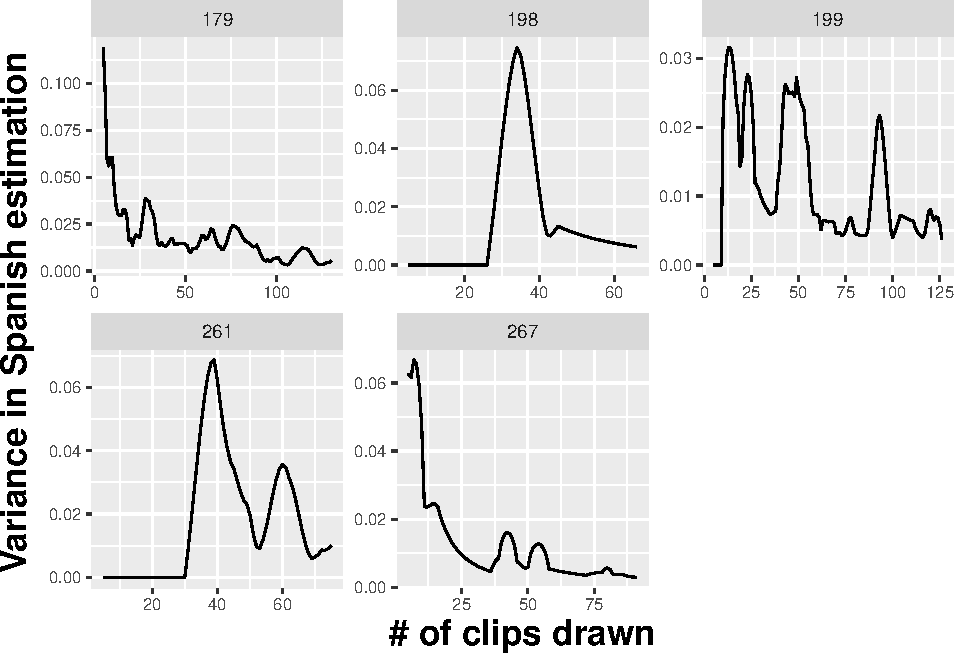
\includegraphics{validation_results_files/figure-latex/plot rolling Spanish variances for US-1.pdf}

\begin{Shaded}
\begin{Highlighting}[]
\KeywordTok{jpeg}\NormalTok{(}\StringTok{"/Users/megcychosz/Google Drive/biling_CDS/results/figures/span_CI_var_plot.jpeg"}\NormalTok{, }\DataTypeTok{height =} \DecValTok{450}\NormalTok{, }\DataTypeTok{width =} \DecValTok{700}\NormalTok{)}
\NormalTok{span_var_plot}
\KeywordTok{dev.off}\NormalTok{()}
\end{Highlighting}
\end{Shaded}

\begin{verbatim}
## pdf 
##   2
\end{verbatim}

\begin{Shaded}
\begin{Highlighting}[]
\NormalTok{que_var <-}\StringTok{ }\NormalTok{random }\OperatorTok\StringTok{ }
\StringTok{  }\KeywordTok{group_by}\NormalTok{(id) }\OperatorTok
\StringTok{  }\KeywordTok{mutate}\NormalTok{(}\DataTypeTok{total=}\KeywordTok{n}\NormalTok{()) }\OperatorTok\StringTok{ }\CommentTok{# total clips drawn }
\StringTok{  }\KeywordTok{filter}\NormalTok{(researcher_present}\OperatorTok{!=}\StringTok{'1'} \OperatorTok{&}\StringTok{ }\NormalTok{sleeping}\OperatorTok{!=}\StringTok{'1'} \OperatorTok{&}\StringTok{ }\NormalTok{percents_voc}\OperatorTok{>}\DecValTok{0}\NormalTok{) }\OperatorTok\StringTok{ }\CommentTok{# criteria for draw, but don't listen}
\StringTok{  }\KeywordTok{distinct}\NormalTok{(file_name, }\DataTypeTok{.keep_all =}\NormalTok{ T) }\OperatorTok
\StringTok{  }\KeywordTok{mutate}\NormalTok{(}\DataTypeTok{annotation_num =} \KeywordTok{as.numeric}\NormalTok{(}\DecValTok{1}\OperatorTok{:}\KeywordTok{n}\NormalTok{())) }\OperatorTok\StringTok{ }\CommentTok{# total clips annotated for lang/reg/childvoc/media, not just drawn}
\StringTok{  }\KeywordTok{gather}\NormalTok{(}\StringTok{"addressee"}\NormalTok{, }\StringTok{"language"}\NormalTok{, Adult2TargetChild, Otherchild2TargetChild, Otherchild2OtherChild, Otherchild2adults,}
\NormalTok{         Otherchild2unsure, Adult2OtherChild, Adult2Others, Adult2unsure) }\OperatorTok
\StringTok{  }\KeywordTok{distinct_at}\NormalTok{(., }\KeywordTok{vars}\NormalTok{(file_name, timestamp_HHMMSS, language), }\DataTypeTok{.keep_all =}\NormalTok{ T) }\OperatorTok\StringTok{ }\CommentTok{# each unique 'language' category only gets counted 1x/clip}
\StringTok{  }\KeywordTok{select}\NormalTok{(}\OperatorTok{-}\NormalTok{addressee)}

\NormalTok{que_var}\OperatorTok{$}\NormalTok{que_cts <-}\StringTok{ }\NormalTok{plyr}\OperatorTok{::}\KeywordTok{mapvalues}\NormalTok{(que_var}\OperatorTok{$}\NormalTok{language, }
                                     \DataTypeTok{from=}\KeywordTok{c}\NormalTok{(}\StringTok{"Categorize language to adults"}\NormalTok{, }\StringTok{"Categorize language to other adults"}\NormalTok{, }
                                            \StringTok{"Categorize language to other child(ren)"}\NormalTok{,}
                                            \StringTok{"Categorize language to someone unknown"}\NormalTok{,}
                                            \StringTok{"Categorize language to target child"}\NormalTok{,}
                                            \StringTok{"Unsure"}\NormalTok{,}
                                            \StringTok{"None"}\NormalTok{, }\StringTok{"English/Quechua"}\NormalTok{, }\StringTok{"Mixed"}\NormalTok{, }\StringTok{"Spanish"}\NormalTok{), }
                                     \DataTypeTok{to=}\KeywordTok{c}\NormalTok{(}\StringTok{"0"}\NormalTok{,}\StringTok{"0"}\NormalTok{,}\StringTok{"0"}\NormalTok{,}\StringTok{"0"}\NormalTok{,}\StringTok{"0"}\NormalTok{,}\StringTok{"0"}\NormalTok{,}\StringTok{"0"}\NormalTok{,}\StringTok{"1"}\NormalTok{, }\StringTok{"0"}\NormalTok{, }\StringTok{"0"}\NormalTok{)) }

\NormalTok{que_var2 <-}\StringTok{ }\NormalTok{que_var }\OperatorTok
\StringTok{  }\KeywordTok{distinct_at}\NormalTok{(., }\KeywordTok{vars}\NormalTok{(file_name, que_cts), }\DataTypeTok{.keep_all =}\NormalTok{ T) }\OperatorTok
\StringTok{  }\KeywordTok{mutate}\NormalTok{(}\DataTypeTok{que_cts =} \KeywordTok{as.numeric}\NormalTok{(que_cts),}
         \DataTypeTok{total =} \KeywordTok{as.numeric}\NormalTok{(total)) }\OperatorTok
\StringTok{  }\KeywordTok{group_by}\NormalTok{(file_name, timestamp_HHMMSS) }\OperatorTok\StringTok{ }
\StringTok{  }\KeywordTok{add_count}\NormalTok{() }\OperatorTok
\StringTok{  }\KeywordTok{filter}\NormalTok{(}\OperatorTok{!}\NormalTok{(n}\OperatorTok{==}\DecValTok{2} \OperatorTok{&}\StringTok{ }\NormalTok{que_cts}\OperatorTok{==}\DecValTok{0}\NormalTok{)) }\OperatorTok\StringTok{ }\CommentTok{# when quechua and another category are marked, only count quechua }
\StringTok{  }\KeywordTok{group_by}\NormalTok{(file_name) }\OperatorTok
\StringTok{  }\KeywordTok{distinct_at}\NormalTok{(., }\KeywordTok{vars}\NormalTok{(annotation_num, language), }\DataTypeTok{.keep_all =}\NormalTok{ T) }\OperatorTok\StringTok{ }\CommentTok{# remove 1 count of quechua (it gets counted 2x when multiple speakers used it)}
\StringTok{  }\KeywordTok{select}\NormalTok{(}\OperatorTok{-}\NormalTok{n)}

\NormalTok{que_rolling <-}\StringTok{ }\NormalTok{que_var2 }\OperatorTok
\StringTok{  }\KeywordTok{filter}\NormalTok{(location}\OperatorTok{==}\StringTok{'Bolivia'}\NormalTok{) }\OperatorTok
\StringTok{  }\KeywordTok{group_by}\NormalTok{(id) }\OperatorTok
\StringTok{  }\KeywordTok{arrange}\NormalTok{(annotation_num) }\OperatorTok
\StringTok{  }\KeywordTok{mutate}\NormalTok{(}\DataTypeTok{que_running_cts =} \KeywordTok{as.numeric}\NormalTok{(}\KeywordTok{cumsum}\NormalTok{(que_cts))) }\OperatorTok
\StringTok{  }\KeywordTok{mutate}\NormalTok{(}\DataTypeTok{roll_prop_que =}\NormalTok{ que_running_cts }\OperatorTok{/}\StringTok{ }\NormalTok{annotation_num,}
         \DataTypeTok{roll_mean_que =} \KeywordTok{rollmean}\NormalTok{(roll_prop_que, }\DataTypeTok{k=}\DecValTok{10}\NormalTok{, }\DataTypeTok{fill =} \OtherTok{NA}\NormalTok{),}
         \DataTypeTok{roll_sd_que =} \KeywordTok{rollapply}\NormalTok{(roll_prop_que, }\DataTypeTok{width=}\DecValTok{10}\NormalTok{, }\DataTypeTok{FUN=}\NormalTok{sd, }\DataTypeTok{fill=}\OtherTok{NA}\NormalTok{))}

\CommentTok{# running binomial confidence interval (wilson)}
\NormalTok{que_rolling2 <-}\StringTok{ }\NormalTok{que_rolling }\OperatorTok
\StringTok{  }\KeywordTok{group_by}\NormalTok{(id, annotation_num) }\OperatorTok\StringTok{ }\CommentTok{# group by id and sample size}
\StringTok{  }\KeywordTok{arrange}\NormalTok{(annotation_num) }\OperatorTok
\StringTok{  }\KeywordTok{summarize}\NormalTok{(}\DataTypeTok{cis =} \KeywordTok{binom.confint}\NormalTok{(que_running_cts, annotation_num, }\DataTypeTok{methods =} \StringTok{'wilson'}\NormalTok{, }\DataTypeTok{conf.level =} \FloatTok{.95}\NormalTok{)) }\OperatorTok
\StringTok{  }\KeywordTok{merge}\NormalTok{(., que_rolling, }\DataTypeTok{by =} \KeywordTok{c}\NormalTok{(}\StringTok{'id'}\NormalTok{, }\StringTok{'annotation_num'}\NormalTok{))}
\end{Highlighting}
\end{Shaded}

\begin{Shaded}
\begin{Highlighting}[]
\NormalTok{que_var_plot <-}\StringTok{ }\NormalTok{que_rolling2 }\OperatorTok
\CommentTok{#filter(roll_sd_que!='NA') %>% # remove rows where variance wasn't estimated}
\StringTok{    }\KeywordTok{mutate}\NormalTok{(}\DataTypeTok{mean_ci =}\NormalTok{ cis}\OperatorTok{$}\NormalTok{mean,}
         \DataTypeTok{upper_ci =}\NormalTok{ cis}\OperatorTok{$}\NormalTok{upper,}
         \DataTypeTok{lower_ci =}\NormalTok{ cis}\OperatorTok{$}\NormalTok{lower) }\OperatorTok\StringTok{  }
\KeywordTok{ggplot}\NormalTok{(., }\KeywordTok{aes}\NormalTok{(annotation_num, roll_prop_que)) }\OperatorTok{+}
\StringTok{  }\KeywordTok{geom_ribbon}\NormalTok{(}\KeywordTok{aes}\NormalTok{(}\DataTypeTok{ymax=}\NormalTok{upper_ci, }\DataTypeTok{ymin=}\NormalTok{lower_ci), }\DataTypeTok{fill=}\StringTok{'lightblue'}\NormalTok{, }\DataTypeTok{color=}\StringTok{'deepskyblue4'}\NormalTok{) }\OperatorTok{+}
\StringTok{  }\KeywordTok{geom_line}\NormalTok{(}\KeywordTok{aes}\NormalTok{(}\DataTypeTok{y=}\NormalTok{mean_ci), }\DataTypeTok{color=}\StringTok{'gray40'}\NormalTok{, }\DataTypeTok{size=}\NormalTok{.}\DecValTok{8}\NormalTok{) }\OperatorTok{+}\StringTok{ }
\StringTok{  }\KeywordTok{xlab}\NormalTok{(}\StringTok{"# of clips annotated"}\NormalTok{) }\OperatorTok{+}\StringTok{ }
\StringTok{  }\KeywordTok{ylab}\NormalTok{(}\StringTok{"Quechua language estimation }\CharTok{\textbackslash{}n}\StringTok{ and variance"}\NormalTok{) }\OperatorTok{+}\StringTok{ }
\StringTok{  }\KeywordTok{facet_wrap}\NormalTok{(}\OperatorTok{~}\NormalTok{id, }\DataTypeTok{scales =} \StringTok{"free"}\NormalTok{) }\OperatorTok{+}
\StringTok{  }\CommentTok{#title = 'Variance in Quechua language estimation as a function of clips drawn: Bolivia corpus') +}
\StringTok{ }\KeywordTok{theme}\NormalTok{(}\DataTypeTok{title =} \KeywordTok{element_text}\NormalTok{(}\DataTypeTok{size=}\DecValTok{12}\NormalTok{),}
   \DataTypeTok{axis.text=}\KeywordTok{element_text}\NormalTok{(}\DataTypeTok{size=}\DecValTok{8}\NormalTok{),}
      \DataTypeTok{axis.title=}\KeywordTok{element_text}\NormalTok{(}\DataTypeTok{size=}\DecValTok{17}\NormalTok{,}\DataTypeTok{face=}\StringTok{"bold"}\NormalTok{),}
      \DataTypeTok{legend.title =} \KeywordTok{element_text}\NormalTok{(}\DataTypeTok{size=}\DecValTok{15}\NormalTok{)) }\OperatorTok{+}
\StringTok{  }\KeywordTok{labs}\NormalTok{(}\DataTypeTok{caption =} \StringTok{"Number of clips annotated refers to those annotated for language, speech register, child vocalizations, and/or media."}\NormalTok{)}
\NormalTok{que_var_plot}
\end{Highlighting}
\end{Shaded}

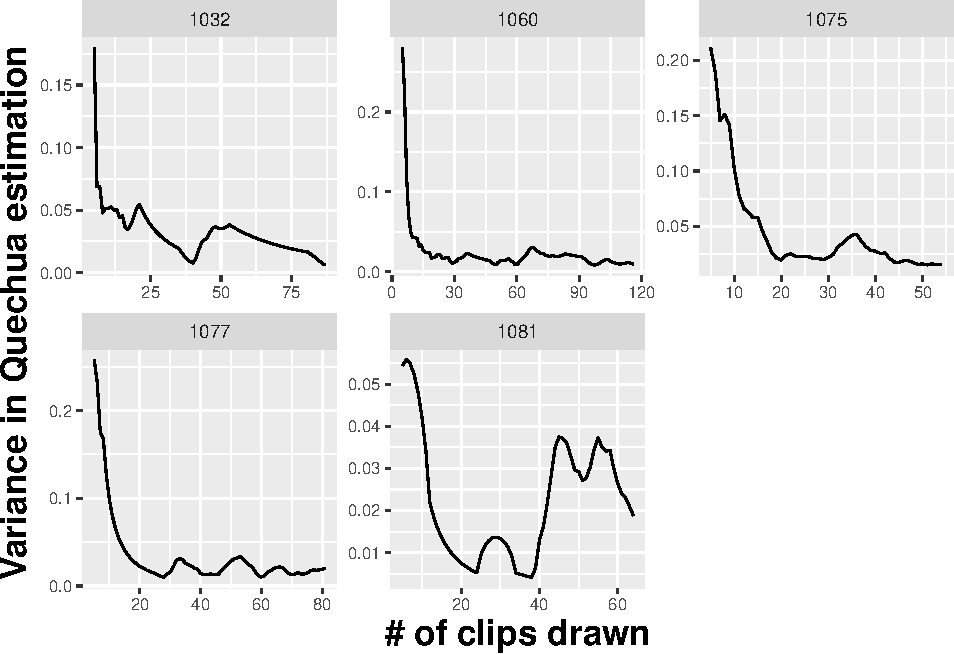
\includegraphics{validation_results_files/figure-latex/plot rolling Quechua variances for Bolivia-1.pdf}

\begin{Shaded}
\begin{Highlighting}[]
\KeywordTok{jpeg}\NormalTok{(}\StringTok{"/Users/megcychosz/Google Drive/biling_CDS/results/figures/que_CI_var_plot.jpeg"}\NormalTok{, }\DataTypeTok{height =} \DecValTok{450}\NormalTok{, }\DataTypeTok{width =} \DecValTok{700}\NormalTok{)}
\NormalTok{que_var_plot}
\KeywordTok{dev.off}\NormalTok{()}
\end{Highlighting}
\end{Shaded}

\begin{verbatim}
## pdf 
##   2
\end{verbatim}

\begin{Shaded}
\begin{Highlighting}[]
\CommentTok{# report CI ranges at 80-clip mark and when annotation stopped, by child}
\NormalTok{que_cis_table <-}\StringTok{ }\NormalTok{que_rolling2 }\OperatorTok
\StringTok{  }\KeywordTok{group_by}\NormalTok{(id) }\OperatorTok
\StringTok{  }\KeywordTok{filter}\NormalTok{(annotation_num}\OperatorTok{==}\DecValTok{80} \OperatorTok{|}\StringTok{ }\NormalTok{annotation_num}\OperatorTok{==}\KeywordTok{NROW}\NormalTok{(id)) }\OperatorTok\StringTok{ }\CommentTok{# get values at 80-clip mark and cut-off}
\StringTok{  }\KeywordTok{mutate}\NormalTok{(}\DataTypeTok{ci_range =}\NormalTok{ cis}\OperatorTok{$}\NormalTok{upper }\OperatorTok{-}\StringTok{ }\NormalTok{cis}\OperatorTok{$}\NormalTok{lower)}

\NormalTok{lang_cis_table <-}\StringTok{ }\NormalTok{span_rolling2 }\OperatorTok
\StringTok{  }\KeywordTok{group_by}\NormalTok{(id) }\OperatorTok
\StringTok{  }\KeywordTok{filter}\NormalTok{(annotation_num}\OperatorTok{==}\DecValTok{80} \OperatorTok{|}\StringTok{ }\NormalTok{annotation_num}\OperatorTok{==}\KeywordTok{NROW}\NormalTok{(id)) }\OperatorTok\StringTok{ }\CommentTok{# get values at 80-clip mark and cut-off}
\StringTok{  }\KeywordTok{mutate}\NormalTok{(}\DataTypeTok{ci_range =}\NormalTok{ cis}\OperatorTok{$}\NormalTok{upper }\OperatorTok{-}\StringTok{ }\NormalTok{cis}\OperatorTok{$}\NormalTok{lower) }\OperatorTok
\StringTok{  }\KeywordTok{rbind}\NormalTok{(., que_cis_table) }\OperatorTok
\StringTok{  }\KeywordTok{select}\NormalTok{(id, annotation_num, ci_range) }\OperatorTok
\StringTok{  }\KeywordTok{mutate}\NormalTok{(}\DataTypeTok{ci_range =} \KeywordTok{round}\NormalTok{(ci_range,}\DecValTok{2}\NormalTok{)) }\OperatorTok
\StringTok{  }\KeywordTok{mutate}\NormalTok{(}\DataTypeTok{timept =} \KeywordTok{if_else}\NormalTok{(annotation_num}\OperatorTok{==}\DecValTok{80}\NormalTok{, }\StringTok{'80-clip_lang'}\NormalTok{, }\StringTok{'Cut-off_lang'}\NormalTok{)) }\OperatorTok
\StringTok{  }\KeywordTok{select}\NormalTok{(}\OperatorTok{-}\NormalTok{annotation_num) }\OperatorTok
\StringTok{  }\KeywordTok{spread}\NormalTok{(}\StringTok{"timept"}\NormalTok{, }\StringTok{"ci_range"}\NormalTok{)}


\NormalTok{final_cis_table <-}\StringTok{ }\NormalTok{cds_rolling2 }\OperatorTok
\StringTok{  }\KeywordTok{group_by}\NormalTok{(id) }\OperatorTok
\StringTok{  }\KeywordTok{filter}\NormalTok{(annotation_num}\OperatorTok{==}\DecValTok{80} \OperatorTok{|}\StringTok{ }\NormalTok{annotation_num}\OperatorTok{==}\KeywordTok{NROW}\NormalTok{(id)) }\OperatorTok\StringTok{ }\CommentTok{# get values at 80-clip mark and cut-off}
\StringTok{  }\KeywordTok{mutate}\NormalTok{(}\DataTypeTok{ci_range =}\NormalTok{ cis}\OperatorTok{$}\NormalTok{upper }\OperatorTok{-}\StringTok{ }\NormalTok{cis}\OperatorTok{$}\NormalTok{lower) }\OperatorTok
\StringTok{  }\KeywordTok{select}\NormalTok{(id, annotation_num, ci_range) }\OperatorTok
\StringTok{  }\KeywordTok{mutate}\NormalTok{(}\DataTypeTok{ci_range =} \KeywordTok{round}\NormalTok{(ci_range,}\DecValTok{2}\NormalTok{)) }\OperatorTok
\StringTok{  }\KeywordTok{mutate}\NormalTok{(}\DataTypeTok{timept =} \KeywordTok{if_else}\NormalTok{(annotation_num}\OperatorTok{==}\DecValTok{80}\NormalTok{, }\StringTok{'80-clip'}\NormalTok{, }\StringTok{'Cut-off'}\NormalTok{)) }\OperatorTok
\StringTok{  }\KeywordTok{select}\NormalTok{(}\OperatorTok{-}\NormalTok{annotation_num) }\OperatorTok
\StringTok{  }\KeywordTok{spread}\NormalTok{(}\StringTok{"timept"}\NormalTok{, }\StringTok{"ci_range"}\NormalTok{) }\OperatorTok
\StringTok{  }\KeywordTok{merge}\NormalTok{(., lang_cis_table, }\DataTypeTok{by=}\StringTok{'id'}\NormalTok{)}

\NormalTok{knitr}\OperatorTok{::}\KeywordTok{kable}\NormalTok{(final_cis_table, }\DataTypeTok{caption =} \StringTok{'Confidence interval range for Spanish/Quechua and child-directed speech estimation, by child, after annotating 80 clips and at annotation cut-off.'}\NormalTok{, }
             \DataTypeTok{booktabs=}\NormalTok{T, }
             \DataTypeTok{row.names =} \OtherTok{FALSE}\NormalTok{, }
             \DataTypeTok{col.names =} \KeywordTok{c}\NormalTok{(}\StringTok{"Child ID"}\NormalTok{, }\StringTok{"80-clip"}\NormalTok{, }\StringTok{"Cut-off"}\NormalTok{, }\StringTok{"80-clip"}\NormalTok{, }\StringTok{"Cut-off"}\NormalTok{)) }\OperatorTok\StringTok{ }\CommentTok{# "}
\StringTok{  }\KeywordTok{kable_styling}\NormalTok{() }\OperatorTok
\StringTok{  }\KeywordTok{add_header_above}\NormalTok{(}\KeywordTok{c}\NormalTok{(}\StringTok{" "}\NormalTok{ =}\StringTok{ }\DecValTok{1}\NormalTok{, }\StringTok{"Language"}\NormalTok{ =}\StringTok{ }\DecValTok{2}\NormalTok{, }\StringTok{"Child-directed speech"}\NormalTok{ =}\StringTok{ }\DecValTok{2}\NormalTok{)) }\OperatorTok
\StringTok{  }\NormalTok{kableExtra}\OperatorTok{::}\KeywordTok{kable_styling}\NormalTok{(}\DataTypeTok{latex_options =} \StringTok{"hold_position"}\NormalTok{)}
\end{Highlighting}
\end{Shaded}

\begin{table}[!h]

\caption{(\#tab:report CI ranges)Confidence interval range for Spanish/Quechua and child-directed speech estimation, by child, after annotating 80 clips and at annotation cut-off.}
\centering
\begin{tabular}[t]{lrrrr}
\toprule
\multicolumn{1}{c}{ } & \multicolumn{2}{c}{Language} & \multicolumn{2}{c}{Child-directed speech} \\
\cmidrule(l{3pt}r{3pt}){2-3} \cmidrule(l{3pt}r{3pt}){4-5}
Child ID & 80-clip & Cut-off & 80-clip & Cut-off\\
\midrule
1032 & 0.16 & 0.12 & 0.21 & 0.17\\
1060 & 0.13 & 0.10 & 0.21 & 0.17\\
1075 & 0.10 & 0.08 & 0.18 & 0.14\\
1077 & 0.11 & 0.09 & 0.21 & 0.17\\
1081 & 0.14 & 0.10 & 0.14 & 0.12\\
\addlinespace
179 & 0.21 & 0.16 & 0.21 & 0.16\\
198 & 0.18 & 0.14 & 0.21 & 0.16\\
199 & 0.20 & 0.16 & 0.17 & 0.15\\
261 & 0.19 & 0.13 & 0.19 & 0.14\\
267 & 0.21 & 0.16 & 0.20 & 0.16\\
\bottomrule
\end{tabular}
\end{table}

\begin{Shaded}
\begin{Highlighting}[]
\CommentTok{# cds model }
\NormalTok{cds_model_data <-}\StringTok{ }\NormalTok{cds_rolling2 }\OperatorTok
\StringTok{  }\KeywordTok{group_by}\NormalTok{(id) }\OperatorTok
\StringTok{  }\KeywordTok{arrange}\NormalTok{(annotation_num) }\OperatorTok
\StringTok{  }\KeywordTok{mutate}\NormalTok{(}\DataTypeTok{halfrow =} \KeywordTok{as.numeric}\NormalTok{(}\KeywordTok{n}\NormalTok{()}\OperatorTok{/}\DecValTok{2}\NormalTok{)) }\OperatorTok\StringTok{ }\CommentTok{# for a sanity check}
\StringTok{  }\KeywordTok{filter}\NormalTok{(}\KeywordTok{row_number}\NormalTok{() }\OperatorTok{>}\StringTok{ }\KeywordTok{n}\NormalTok{()}\OperatorTok{*}\NormalTok{.}\DecValTok{50}\NormalTok{) }\CommentTok{# get the top 10% of rows from each group}
  
\NormalTok{cds_model <-}\StringTok{ }\NormalTok{cds_model_data }\OperatorTok
\StringTok{  }\CommentTok{#filter(roll_sd_cds!='NA') %>%}
\StringTok{  }\KeywordTok{filter}\NormalTok{(location}\OperatorTok{==}\StringTok{'US'}\NormalTok{) }\OperatorTok
\StringTok{  }\KeywordTok{mutate}\NormalTok{(}\DataTypeTok{ci_range =}\NormalTok{ cis}\OperatorTok{$}\NormalTok{upper }\OperatorTok{-}\StringTok{ }\NormalTok{cis}\OperatorTok{$}\NormalTok{lower) }\OperatorTok\StringTok{ }
\StringTok{  }\KeywordTok{lmer}\NormalTok{(ci_range}\OperatorTok{~}\NormalTok{annotation_num }\OperatorTok{+}\StringTok{ }\NormalTok{(}\DecValTok{1}\OperatorTok{|}\NormalTok{id), }\DataTypeTok{data =}\NormalTok{ .) }\OperatorTok
\StringTok{  }\KeywordTok{summary}\NormalTok{()}

\CommentTok{# spanish model}
\CommentTok{# redo data to get the Bolivia corpus at the same time (more power for stats)}
\NormalTok{span_rolling_all <-}\StringTok{ }\NormalTok{span_var2 }\OperatorTok
\StringTok{  }\KeywordTok{group_by}\NormalTok{(id) }\OperatorTok\StringTok{ }
\StringTok{  }\KeywordTok{arrange}\NormalTok{(annotation_num) }\OperatorTok
\StringTok{  }\KeywordTok{mutate}\NormalTok{(}\DataTypeTok{span_running_cts =} \KeywordTok{as.numeric}\NormalTok{(}\KeywordTok{cumsum}\NormalTok{(span_cts))) }\OperatorTok
\StringTok{  }\KeywordTok{mutate}\NormalTok{(}\DataTypeTok{roll_prop_span =}\NormalTok{ span_running_cts }\OperatorTok{/}\StringTok{ }\NormalTok{annotation_num,}
         \DataTypeTok{roll_mean_span =} \KeywordTok{rollmean}\NormalTok{(roll_prop_span, }\DataTypeTok{k=}\DecValTok{10}\NormalTok{, }\DataTypeTok{fill =} \OtherTok{NA}\NormalTok{),}
         \DataTypeTok{roll_sd_span =} \KeywordTok{rollapply}\NormalTok{(roll_prop_span, }\DataTypeTok{width=}\DecValTok{10}\NormalTok{, }\DataTypeTok{FUN=}\NormalTok{sd, }\DataTypeTok{fill=}\OtherTok{NA}\NormalTok{)) }

\CommentTok{# running binomial confidence interval (wilson)}
\NormalTok{span_rolling_all2 <-}\StringTok{ }\NormalTok{span_rolling_all }\OperatorTok
\StringTok{  }\KeywordTok{group_by}\NormalTok{(id, annotation_num) }\OperatorTok\StringTok{ }\CommentTok{# group by id and sample size}
\StringTok{  }\KeywordTok{arrange}\NormalTok{(annotation_num) }\OperatorTok
\StringTok{  }\KeywordTok{summarize}\NormalTok{(}\DataTypeTok{cis =} \KeywordTok{binom.confint}\NormalTok{(span_running_cts, annotation_num, }\DataTypeTok{methods =} \StringTok{'wilson'}\NormalTok{, }\DataTypeTok{conf.level =} \FloatTok{.95}\NormalTok{)) }\OperatorTok
\StringTok{  }\KeywordTok{merge}\NormalTok{(., span_rolling_all, }\DataTypeTok{by =} \KeywordTok{c}\NormalTok{(}\StringTok{'id'}\NormalTok{, }\StringTok{'annotation_num'}\NormalTok{)) }

\CommentTok{# fit the spanish models}
\NormalTok{span_model_data <-}\StringTok{ }\NormalTok{span_rolling_all2 }\OperatorTok
\StringTok{  }\KeywordTok{group_by}\NormalTok{(id) }\OperatorTok
\StringTok{  }\KeywordTok{arrange}\NormalTok{(annotation_num) }\OperatorTok
\StringTok{  }\KeywordTok{mutate}\NormalTok{(}\DataTypeTok{halfrow =} \KeywordTok{as.numeric}\NormalTok{(}\KeywordTok{n}\NormalTok{()}\OperatorTok{/}\DecValTok{2}\NormalTok{)) }\OperatorTok\StringTok{ }\CommentTok{# for a sanity check}
\StringTok{  }\KeywordTok{filter}\NormalTok{(}\KeywordTok{row_number}\NormalTok{() }\OperatorTok{>}\StringTok{ }\KeywordTok{n}\NormalTok{()}\OperatorTok{*}\NormalTok{.}\DecValTok{50}\NormalTok{)}

\NormalTok{span_model <-}\StringTok{ }\NormalTok{span_model_data }\OperatorTok
\StringTok{  }\CommentTok{#filter(roll_sd_span!='NA') %>%}
\StringTok{  }\KeywordTok{mutate}\NormalTok{(}\DataTypeTok{ci_range =}\NormalTok{ cis}\OperatorTok{$}\NormalTok{upper }\OperatorTok{-}\StringTok{ }\NormalTok{cis}\OperatorTok{$}\NormalTok{lower) }\OperatorTok\StringTok{ }\CommentTok{# get the variance}
\StringTok{  }\KeywordTok{lmer}\NormalTok{(ci_range}\OperatorTok{~}\NormalTok{annotation_num }\OperatorTok{+}\StringTok{ }\NormalTok{(}\DecValTok{1}\OperatorTok{|}\NormalTok{id), }\DataTypeTok{data =}\NormalTok{ .) }\OperatorTok
\StringTok{  }\KeywordTok{summary}\NormalTok{()}
\end{Highlighting}
\end{Shaded}

\end{document}
